\documentclass{report}
\usepackage[utf8]{inputenc}

% Style and margins:
\usepackage{geometry}
\geometry{
    a4paper,
    left=30mm,
    right=30mm,
    top=25mm,
    bottom=25mm,
    twoside
}
\setlength{\parskip}{3mm}
\usepackage{url}
\usepackage{times}
\pagestyle{plain}

\usepackage{titlesec}
\titleformat{\chapter}
  {\normalfont\Huge\bfseries}{\thechapter}{1em}{}

% For figures:
\usepackage{graphicx}
\usepackage{float}
\graphicspath{ {Figures/} }
\renewcommand{\figurename}{Fig.}

% For source code:
\usepackage{listings}
\usepackage{xcolor}

\lstset{
  frame=tb,
  basicstyle=\footnotesize\ttfamily,
  language=C++,
  numbers=left,
  numbersep=5pt,
  breaklines=true,
  extendedchars=true,
  literate={ñ}{{\~n}}1
}

% Math
\usepackage{amsmath}

%Bibliography
\usepackage[style=verbose-ibid, backend=biber,sorting=none]{biblatex}
\bibliography{Bibliography}

% Data
%Desenvolupament d'aplicació 3D per escriptori i web mitjançant Emscripten
%Development of 3D application for desktop and web using Emscripten
\title{Desarrollo de aplicación 3D para escritorio y web mediante Emscripten}
\author{Daniel Barca Casafont}
\date{Junio de 2017}

%%%%%%%%%%%%%%%%%%%%%%%%%%%%%%%%%%%%%%%%%%%%%%%%%
\begin{document}

\pagenumbering{roman}
\begin{titlepage}
\maketitle
\end{titlepage}

\cleardoublepage
\renewcommand{\contentsname}{Índice}
\tableofcontents

\cleardoublepage
\begin{abstract}
En este documento se recoge el proceso de desarrollo de una aplicación 3D multiplataforma para la empresa Interiorvista, la cual permite configurar y visualizar estancias con el lenguaje de programación C++ dados unos requerimientos inciales. Haciendo uso de Emscripten, el código ha sido adaptado a las limitaciones de las plataformas web que no encontramos en aplicaciones de escritorio tradicionales, tales como la existencia de un único hilo de ejecución o la ausencia de un sistema de ficheros. También se deberá adaptar el motor gráfico de la empresa para que funcione mediante WebGL o Vulkan en función de la plataforma donde se ejecute. Además, se discuten detalles sobre el diseño de software y el proceso de desarrollo de la aplicación en sí.

This document describes the process of developing a 3D multiplatform application for the company Interiorvista, that allows users to configure and visualize rooms with the C++ programming language given some initial requirements. Using Emscripten, the code has been adapted to the limitations of web platforms that are not found in traditional desktop applications, such as the existence of only one single execution thread or the absence of a file system. The company's graphics engine must also be adapted in order to work using WebGL or Vulkan depending on the platform where it's running. In addition, this document discusses details about the software design and the development process of the application itself.
\end{abstract}

\cleardoublepage
\renewcommand{\listfigurename}{Lista de Figuras}
\listoffigures

\cleardoublepage
\pagenumbering{arabic}

\chapter{Introducción}
\section{Motivación}
Interiorvista es una empresa especializada en la generación de imágenes por computador (mucho más baratas, rápidas y de igual o mejor calidad que las que pueden obtenerse con un plató y un fotógrafo) y en el desarrollo de aplicaciones web (que requieren personal muy especializado y una gran inversión de tiempo).

Entre estas aplicaciones se encuentran los \textit{Interiorvista Planner}, un conjunto de aplicaciones que tienen el objetivo de permitir a los usuarios generar habitaciones tridimensionales y poblarlas con los productos que los clientes ofrecen en su catálogo. Esto plantea una serie de retos a varios niveles.

En su estado actual, las aplicaciones desarrolladas tienen problemas que hacen cada vez más difícil el mantenimiento y la mejora de estas. Muchas de sus características han sido desarrolladas sin llevar a cabo ningún diseño previo, o incluso sin una especificación previa de los requerimientos de la aplicación, provocando que estos surjan a lo largo del desarrollo.

\begin{figure}[H]
    \centering
    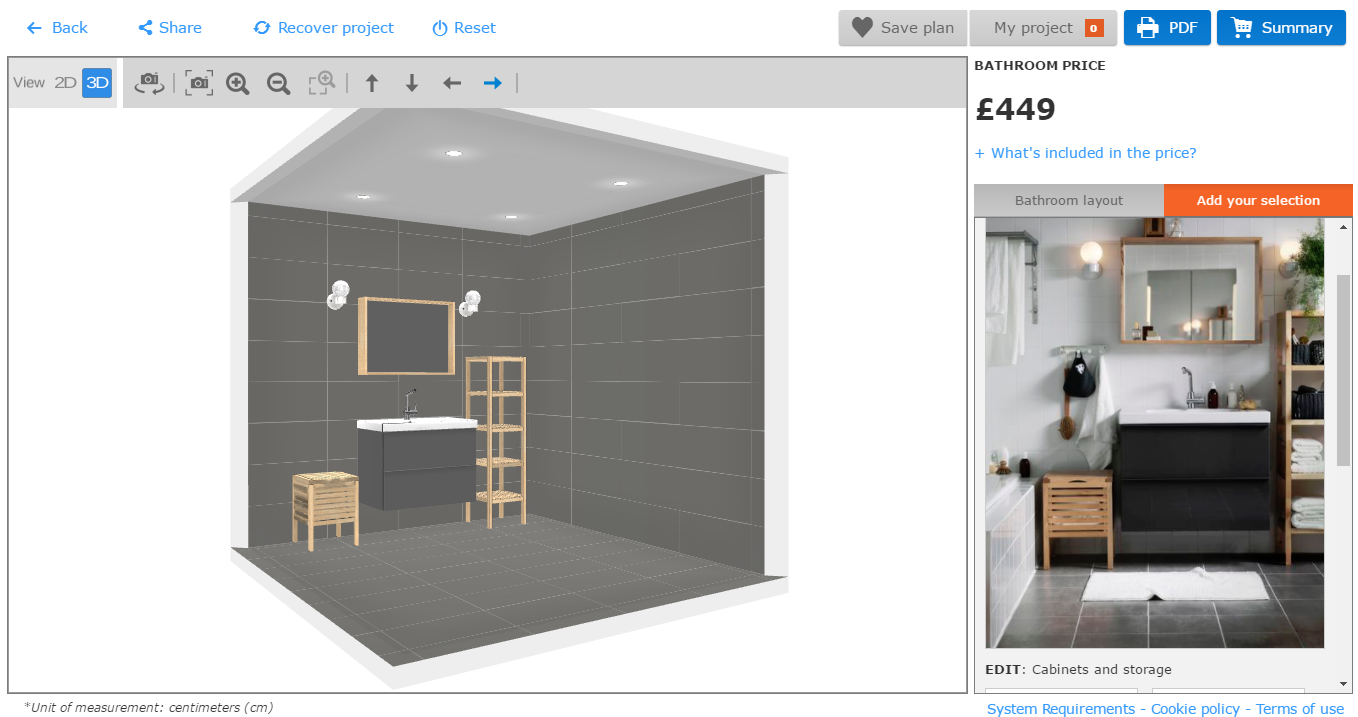
\includegraphics[width=0.8\linewidth]{bathroom_vista}
    \caption{Versión actual del planificador Bathroom Vista en vista 3D.}
    \label{fig:bathroom_vista}
\end{figure}


Las compañías de interiorismo suelen tener una serie de normas por las cuales ciertos elementos estructurales no pueden introducirse en ciertas combinaciones o en ciertas posiciones. Esto ha llevado a un código demasiado especializado en el que se introducen excepciones y condiciones arbitrarias sin mucho orden.

Se suelen requerir diversas aplicaciones muy similares para los distintos ambientes que ofrecen en su catálogo: habitaciones, comedores, baños, cocinas, etc. Aunque cada caso tiene sus particularidades, en general la mayoría de planificadores tienen suficientes características comunes como para poder tener un núcleo común, cosa que no está ocurriendo en estos momentos.

Generalmente casi siempre vamos a tener una habitación con ventanas, puertas, y una serie de elementos interiores que podemos distribuir por esta. Por ello, con un diseño efectivo debe ser posible reducir la especialización de cada una de estas aplicaciones. En el futuro, una posibilidad con la que se ha soñado en Interiorvista es la de hacer un planificador completo de una planta, con todas sus habitaciones, algo que no resultaría sencillo de conseguir con los desarrollos de que disponemos actualmente.

Entre las características comunes de los planificadores encontramos que la mayoría disponen de un modo visualización en 2 dimensiones, pensado para configurar la estructura de una habitación, y otro en 3 dimensiones, pensado para visualizar el resultado y realizar retoques sobre este. En estos momentos estos modos se han programado como dos programas distintos con una parte 2D hecha con tecnologías web, y una 3D hecha con un motor gráfico exportado a WebGL. Es una duplicidad de esfuerzos que puede evitarse utilizando una cámara ortogonal en 3D y algunas modificaciones visuales.

\begin{figure}[H]
    \centering
    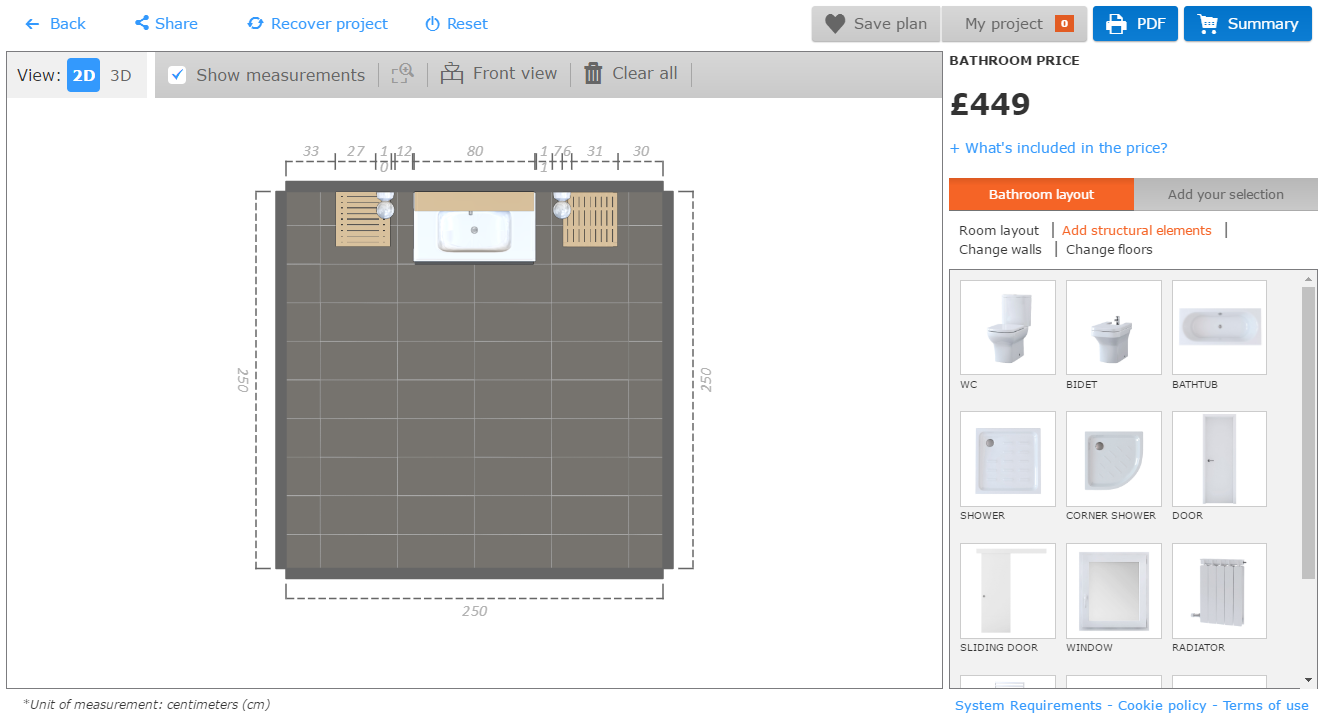
\includegraphics[width=0.8\linewidth]{bathroom_vista_2d}
    \caption{Bathroom Vista, versión en dos dimensiones del baño en la figura \ref{fig:bathroom_vista}.}
    \label{fig:bathroom_vista_2d}
\end{figure}

A pesar de las similitudes siempre hay elementos que hacen único a cada Planner: algunos baños o cocinas tienen diferentes texturas combinables para las paredes, algunas habitaciones tienen un techo inclinado o algunos productos de son altamente configurables y requieren más atención. Diferentes planificadores pueden tener un enfoque distinto: desde completas herramientas que han de poder generar y visualizar todas las configuraciones posibles de una estancia hasta aplicaciones que buscan un enfoque más emocional que atraiga a los usuarios, lo cual implica sacrificar funcionalidad en favor de la estética. Incluso pueden llegar a existir dos aplicaciones para un mismo conjunto de productos, con el objetivo de cubrir ambos puntos de vista.

El hecho de estar utilizando motores gráficos propietarios nos ha provocado problemas en el pasado. Las necesidades de la empresa son muy específicas y la imposibilidad de controlar el funcionamiento del motor ha hecho que no podamos solucionar efectivamente muchos problemas, llevándonos incluso a tener que esperar a que los desarrolladores lancen actualizaciones que arreglen nuestros problemas, o a mantener versiones abandonadas porque las versiones nuevas no son compatibles con ciertos requerimientos.

La falta de control sobre el motor gráfico también ha hecho que no pudiéramos realizar ciertas mejoras de eficiencia, visualización, o reducir el peso de la aplicación (por ejemplo, las versiones actuales incluyen toda una API de audio que no es necesaria).

\section{Objetivos}

La aplicación debe ser lo bastante genérica como para aplicarse a diferentes casos, de ahí que digamos que se trata de un conjunto de aplicaciones; y al mismo tiempo también ha de ser flexible como para dar cabida a todas estas características.

Debe contar con un visualizador en 2 y 3 dimensiones. Según el modo de visualización la interacción y las opciones son diferentes, pero el estado y la lógica de la aplicación debe mantenerse el máximo posible.

A largo plazo, la aplicación debe poder ejecutarse sobre distintas plataformas como web, escritorio, móviles o tabletas. Esto tiene muchas implicaciones a nivel de software e interacción: distintas plataformas cuentan con distintos drivers y APIs de ejecución y cada una tiene un funcionamiento y un modo de uso muy distinto. Dado que la aplicación va a estar completamente programada en C++, trasladar el código a otras plataformas (especialmente web) puede suponer un reto.

El desarrollo se realizará sobre un motor gráfico propio de la empresa, el cual está pensado para funcionar con la API gráfica Vulkan en escritorio, y debe ser adaptado para poder utilizarse con otras APIs en otras plataformas como Web o plataformas móviles. El hecho de disponer de un motor gráfico propio nos da un gran control sobre lo que ocurra dentro de este, en contraste con otras alternativas propietarias que no podemos controlar. En el pasado se han tenido muchos problemas haciendo funcionar las aplicaciones en distintas plataformas.

A nivel de diseño de software, esta es una oportunidad para repensar y reorganizar los problemas que ya conocemos. Aplicar correctamente diversas técnicas de diseño de software hará que no sólo sea más sencillo desarrollar la aplicación sino que sea más fácil de mantener y ampliar en el futuro. Algunas características son muy difíciles de implementar si no se ha seguido un cierto diseño desde el principio.

\section{Estado del arte}
Aunque existen diversos planificadores de estancias en el mercado, a día de hoy la mayoría tienen serias deficiencias y prácticamente ninguno está asociado a marcas importantes del modo en que lo está Interiorvista. Sin embargo, eso no impide que aprendamos de las alternativas existentes.

Entre los fallos más comunes se encuentran:
\begin{itemize}
    \item La necesidad de descargar aplicaciones de escritorio, o un gran número de assets que no necesariamente van a utilizarse.
    \item El uso de tecnologías obsoletas, especialmente Adobe Flash (muy popular durante la última década pero en desuso hoy en día), o motores web que requieren la instalación de plugins o extensiones.
    \item Sólo modo en 2 dimensiones o 3 dimensiones, sin la posibilidad de cambiar.
    \item Mala calidad gráfica.
    \item Interacción y/o diseño pobre.
\end{itemize}

Por supuesto, tenemos como precedente los anteriores planificadores hechos en Interiorvista, que aunque están bien situados en el mercado sufren de algunos de los fallos ya mencionados. La alternativa más sólida para lo que queremos realizar es Planner5D\footfullcite{planner5d}, que cumple buena parte de los requerimientos que queremos cumplir; sin embargo a día de hoy también tiene defectos en estabilidad e interacción, como que los elementos interiores no se adhieren a las paredes (a excepción de elementos estructurales de las paredes, como puertas y ventanas), o que en 2D pueden estropearse las paredes de forma relativamente fácil.

%Los planificadores de 2020\cite{2020} se caracterizan entre otras cosas por ofrecer imágenes estáticas de mayor calidad. El planificador espera a que el usuario deje de interactuar con la escena para generar la imagen y sobreponerla al canvas 3D. Aunque funciona, probablemente no se trata de la mejor aproximación a este problema, dado que el resultado no deja de ser un tanto pobre para la cantidad de trabajo que han realizado: generar un render 3D de buena calidad en la nube tiene un gran coste computacional (y por extensión, económico, pues los servidores gráficos son especialmente costosos), por lo que generar un render nuevo cada pocos segundos es inviable. Para solventarlo han reducido la calidad igualmente haciendo que, si bien se ve mejor que el render local, sigue dejando mucho que desear. Además, a nivel de interacción puede resultar engorroso notar el cambio de calidad constantemente.

%Generar imágenes de alta calidad en tiempo real no deja de ser una opción interesante, pero vale la pena considerar otras como mantener el renderizado local hasta que el usuario haya terminado de configurar su habitación, para finalmente generar una o varias imágenes de alta calidad.

\cleardoublepage
\chapter{Descripción del proyecto}
\textit{Interiorvista Planner} es una herramienta que permite crear de forma rápida y fácil el diseño de una sala a medida. Está pensada para ser genérica, de modo que después el proyecto se subdivide en otras aplicaciones.

La aplicación debe permitir configurar las dimensiones y forma de una sala para después introducir elementos propios de cada proyecto en esta, para finalmente obtener un listado de los productos introducidos, el precio de comprar dicha configuración, y un código que permite acceder al proyecto desde una tienda física para realizar la compra.

\section{Clientes}
IKEA\cite{ikea_history} es una archiconocida multinacional especializada en la venta de muebles de bajo coste. Se gestó en Suecia en el año 1943 como una tienda de venta de productos varios para el día a día a un precio reducido, y cuenta hoy con 314 tiendas repartidas en 38 países, siendo el icono más reconocible en el mundo de los muebles.

Una de las claves del éxito de IKEA es su famoso catálogo, donde los potenciales clientes podían ver los muebles que se ofertan y sus posibles distribuciones. Durante los años 2000 IKEA ha puesto su catálogo a disposición de los clientes también a través de Internet, y les ha ofrecido nuevas herramientas con las que poder imaginar cómo van a quedar los productos que compren en su hogar.

ROCA\cite{roca_history} es el principal proveedor de productos para baños del mundo. Se gestó en Gavá en 1917 como una compañía de radiadores, pero su relación con el agua hizo que se interesara rápidamente en la fabricación de porcelana en 1936 y grifería en 1954.

Al igual que IKEA, ROCA ha encontrado en internet nuevas formas de llegar a sus clientes, creando catálogos online y herramientas de configuración y visualización.

Aunque estos son los dos principales clientes de Interiorvista, la naturaleza genérica del planificador hace que cualquier empresa especializada en el interiorismo sea un potencial cliente.

\section{Objetivo del producto}
Los productos de interiorismo destacan por ser altamente configurables y modulares, para adaptarse a los gustos y necesidades de cada comprador. Esto hace que sea complejo crear una aplicación que tenga en cuenta todas las peculiaridades de los productos. Con los \textit{Interiorvista Planner} los compradores deben poder probar y visualizar las diferentes configuraciones de los productos y realizar la compra (a través del código) si así lo deciden.

Por lo tanto, el objetivo es conseguir que un máximo número de clientes generen un código y lo recuperen desde una tienda (signo de que han acabado comprado el producto). Cuanto más satisfactorio sea el proceso de configuración, más probable es que dichos clientes lleguen hasta el final, es por esto que la usabilidad y los tiempos de carga son clave.

Otro objetivo indirecto es hacer que la aplicación sea lo suficientemente genérica como para poder adaptarse, con poco esfuerzo, a los diferentes sub-proyectos.

\section{Usuarios}
Hay dos posibles usuarios de la aplicación: los compradores, que pueden acceder a esta a través de la página web del cliente, desde los ordenadores disponibles en las tiendas o bien desde las aplicaciones móviles; y los empleados del cliente (también conocidos como coworkers), que se encuentran en las tiendas vendiendo productos y ayudando a los clientes.

El enfoque para cada cliente es algo distinto. En el caso de los compradores se busca algo más rápido y emocional, que le lleve lo más rápido posible a la compra del producto. Sin embargo, para los trabajadores esta aplicación es una completa y precisa herramienta de trabajo, que ha de ser capaz de poder reflejar cualquier posible configuración.

A pesar de esto la aplicación será razonablemente similar en ambos casos, a excepción de algunos ``atajos" con los que los trabajadores podrán llegar más rápido a las secciones que les interesan.


\cleardoublepage
\chapter{Motor gráfico}
Como se ha mencionado anteriormente, el motor gráfico con el que trabajaremos para crear esta aplicación es propio de la empresa: Manta. Manta está programado en C++ y pretende ser un motor multipropósito, aunque el hecho de estar programado en la misma empresa nos permite prestar especial atención a los usos específicos que le demos dentro de esta. En este apartado discutiremos algunas de las características más relevantes del motor para con la aplicación. No se pretende pues crear una documentación completa de este sino tan sólo una visión general, como referencia para el desarrollo de la aplicación.

\section{Diseño de software}
\section{APIs gráficas}
\label{APIS}

Según la plataforma en que se esté ejecutando la aplicación, se hará uso de una API gráfica u otra. Por defecto Manta ha sido desarrollado para funcionar en escritorio haciendo uso de Vulkan, pero esta API no está disponible en web, por lo que tendremos que utilizar OpenGL ES 2 y WebGL en este caso. Con este capítulo se pretende mostrar una vista general y con poco detalle de las APIs gráficas consideradas para hacer funcionar el motor en cada plataforma.

\subsection{Vulkan}
\label{vulkan_api}
Entre las diferentes APIs gráficas que existen, la tendencia actual es la de dar cada vez más control al desarrollador sobre lo que ocurre entre la aplicación y la gráfica, dando acceso de bajo nivel al hardware. Vulkan es la respuesta de software libre a esta tendencia, y una de las APIs que más tracción está recogiendo últimamente.

Al ofrecer control de bajo nivel, con Vulkan pueden realizarse muchas optimizaciones que en una API de alto nivel no sería posible realizar\footfullcite{vulkan_spec}. Vulkan facilita el uso de múltiples dispositivos de hardware con diversos propósitos (la GPU puede utilizarse también para realizar cálculos en paralelo, sin estar necesariamente renderizando) y el uso de multithreading.

Para ello Vulkan puede detectar y listar los dispositivos de hardware que se encuentran disponibles en la máquina, así como sus capacidades y especificaciones. Por cada dispositivo se crea una cola de comandos, que describen las acciones a realizar por el hardware.

Los comandos pueden tener distintos estados que permiten controlar el flujo de la aplicación, especialmente en aplicaciones multinúcleo. Dicho estado indica si el comando se ha ejecutado, está a la espera de ejecutarse o está disponible para ser ejecutado de nuevo. Por supuesto, la pipeline gráfica se ejecuta a través de dichos comandos.

En cuanto a la gestión de memoria, Vulkan asigna dos tipos de memoria al dispositivo: una mayor cantidad para los elementos con los que ha de trabajar constantemente, que cambiará lo mínimo posible, y que es inaccesible desde fuera del dispositivo; y otra menor conocida como ``staging" que permite hacer una copia de fragmentos de la memoria principal y modificarlos desde el exterior, para subirlos de nuevo a la principal posteriormente. Este paso se realiza porque es muy ineficiente que un dispositivo acceda a la memoria de la CPU y vice-versa, tanto la GPU como la CPU deben trabajar con su propia memoria y reducir al mínimo la transmisión de datos.

Al contrario que otras APIs, en Vulkan es posible utilizar multithreading. En caso de utilizarse, esto implica la necesidad de controlar la sincronía de cuanto ocurre en la aplicación, pero resulta una gran ventaja si se está dispuesto a realizar el esfuerzo, y supone un mucho mejor aprovechamiento de la CPU teniendo en cuenta que cada vez tienen más núcleos de procesador.

Como puede verse, en Vulkan la aplicación es responsable de la mayor parte de gestión en cuanto a qué debe hacer el dispositivo en cada momento. Es algo que contrasta, como se ha dicho, con la tendencia que ha existido hasta el momento de abstraer los elementos descritos en este apartado. 

Aunque a priori el tener más control resulta beneficioso, se debe tener especial cuidado pues la dificultad de hacer funcionar Vulkan es muy superior que con otras APIs (como OpenGL en el apartado \ref{opengl_webgl_api}), llegando al extremo en que una mala implementación en Vulkan puede dar peores resultados que su equivalente en alternativas que habrían sido mucho más simples de implementar.

\subsection{OpenGL ES 2 y WebGL}
\label{opengl_webgl_api}
En estos momentos en las tecnologías web, WebGL es la única API 3D estándar y por lo tanto que vale la pena considerar. Por eso Vulkan sólo se va a utilizar en escritorio. En el capítulo \ref{emscripten_gapi} se explicará como hacer que una aplicación programada con Vulkan pueda trabajar con WebGL al cambiar a la plataforma web.

OpenGL nació en 1992 como alternativa a las APIs gráficas propietarias del momento. La especificación y estandarización hicieron que se popularizara hasta ser la API gráfica más popular \footfullcite{opengl_hist}. OpenGL ES es una versión de OpenGL para dispositivos embebidos.

WebGL apareció de la necesidad de tener un estándar de aceleración gráfica dentro de las tecnologías web. Hasta el momento las alternativas pasaban por el uso de plugins como Adobe Flash\footfullcite{stage3D_flash}. Está basado en OpenGL ES 2 y su especificación es prácticamente idéntica, de ahí que resulte relativamente sencillo convertir llamadas a OpenGL en llamadas a WebGL.

Al contrario de lo que ocurría con Vulkan en el apartado \ref{vulkan_api}, OpenGL está pensado para proporcionar la mayor sencillez de uso posible, en detrimento del control que posee el desarrollador sobre lo que ocurre a bajo nivel. En OpenGL no es necesario especificar qué dispositivo utilizar (de hecho es prácticamente imposible escoger el dispositivo, lo cual puede ser una desventaja), gestionar la memoria, o manejar los comandos ejecutados por el dispositivo.

Aunque técnicamente es posible hacer programas con múltiples hilos de ejecución con OpenGL, hacerlo no supone ninguna mejora en términos de eficiencia y supone un esfuerzo fútil\footfullcite{opengl_multithreading}. En cualquier caso, la imposibilidad de usar hilos de ejecución en Javascript hace que no podamos aprovechar multithreading de ningún modo con WebGL (véase el apartado \ref{init_emscripten} donde se explican, entre otras cosas, algunas características de Javascript).

El resultado es una mayor rapidez de desarrollo y un código mucho más ligero y sencillo de estructurar en comparación con Vulkan, en consecuencia más fácil de mantener. A pesar de sus limitaciones, por lo general es suficiente para la mayoría de aplicaciones 3D. Para aplicaciones en las cuales el rendimiento sea crítico, sus limitaciones pueden llegar a ser un problema, o al menos una desventaja importante.

\subsection{Otras plataformas}
Aunque en este documento sólo se profundiza en el desarrollo para escritorio y web, en el futuro se espera poder exportar a otras plataformas como sistemas operativos móviles. En este área hay algunas diferencias entre los diferentes proveedores de dispositivos móviles.

A día de hoy, dispositivos con iOS de Apple son compatibles con las versiones de OpenGL ``OpenGL ES 1.1", ``OpenGL ES 2.0" y ``OpenGL ES 3.0" \footfullcite{apple_dev_opengl} mientras que en Android de Google se acepta ``OpenGL ES 1.0", ``OpenGL ES 2.0", ``OpenGL ES 3.0" y ``OpenGL ES 3.1" \footfullcite{google_dev_opengl}. Cada versión de OpenGL tiene ciertas características que mejoran a la anterior aunque hacer uso de estas suele dar problemas de incompatibilidad con las anteriores (las versiones previas de cada sistema operativo puede tener menos versiones de OpenGL compatibles).

Android dispone de una versión de Vulkan pensada especialmente para dispositivos móviles\footfullcite{android_vulkan}, por lo que la exportación de código a Android debería ser relativamente directa. iOS en cambio dispone de su propia API para gráficos de bajo nivel: Metal. Metal comparte gran parte de la filosofía de Vulkan, pero realizar la exportación podría implicar bastante más esfuerzo. No hay expectativas de que Apple incluya soporte a Vulkan dentro de iOS a corto plazo.

Microsoft también cuenta con su propia API gráfica, DirectX, aunque los dispositivos móviles con Windows representan hoy en día una parte marginal del mercado, y es poco probable que valga la pena el esfuerzo de portar el código. Al igual que Vulkan y Metal, DirectX tiene un planteamiento de bajo nivel, aunque su trayectoria es mucho más larga que los dos primeros (su primera versión data de 1995), y sus versiones anteriores no contaban con esta filosofía. DirectX tiene una mayor compatibilidad con dispositivos de escritorio que Vulkan, por lo que podría llegar a ser necesario portar el código a DirectX si en algún momento se requiere ejecutar en un dispositivo Windows que no acepte Vulkan (algunos clientes usan dispositivos muy específicos).

\section{Shaders}

\cleardoublepage
\chapter{Compilación a web con Emscripten}
Uno de los puntos fuertes de nuestro planner es el poder ejecutarlo en web. El hecho de estar programado en C++, sin embargo, dificulta esta tarea. Teniendo cuenta una serie de consideraciones, es posible adaptar código C++ a web a través de Emscripten.

\label{emscripten}
\section{Consideraciones previas}
En esta sección se describen diversas consideraciones que se han tenido en cuenta a la hora de adaptar el código con Emscripten.

%%%%%%%%%%%%%%%%%%%%%%%%%%%%%%%%%%%%%%%%%%%%%%%%%%%%%%%%%%%%%%%%%%%%%%%%%%%%%
%%%%%%%%%%%%%%%%%%%%%%%%%%%%%%%%%%%%%%%%%%%%%%%%%%%%%%%%%%%%%%%%%%%%%%%%%%%%%
%%%%%%%%%%%%%%%%%%%%%%%%%%%%%%%%%%%%%%%%%%%%%%%%%%%%%%%%%%%%%%%%%%%%%%%%%%%%%

\subsection{Sobre Emscripten}
\label{about_emscripten}
Emscripten es capaz de compilar código IL (Intermediate Language) a Javascript. IL es un lenguaje de código máquina que se puede generar compilando desde otros lenguajes, entre ellos C++ usando el compilador LLVM. Dado que Emscripten compila desde IL (y no C++ directamente) realmente esto significa que podemos ejecutar código escrito en diversos lenguajes a través de Emscripten.

Emscripten\footfullcite{kripken_cppcon} nació como respuesta a la necesidad de escribir programas para web en lenguajes tradicionales de escritorio, con el objetivo de ganar velocidad, trabajar con un lenguaje familiar, y aprovechar las librerías existentes en dichos lenguajes. Hasta su aparición la única alternativa para poder hacer esto era el uso de plugins embebidos en el navegador, lo cual fracasó debido a la falta de estandarización y a la evolución de los propios navegadores, que cada vez más rechazan los plugins desde la popularización de las plataformas móviles.

Dada la extensión de funcionalidades de Javascript, para realizar el compilado se ha utilizado un subset de este, ``asm.js". Asm.js es un lenguaje intermedio que podemos ejecutar en navegadores; tiene una serie de restricciones con respecto a Javascript, como por ejemplo el hecho de ser un lenguaje tipado (aunque Javascript no lo es, en asm.js se comprueba el tipo de cada variable antes de trabajar con ella) o el requerimiento de trabajar sobre una única pila de memoria (un simple array de Javascript dentro del cual deben estar todos los datos que utilice el programa).

Si se aplica esta filosofía al código que programamos en C++, se puede entender fácilmente que dicha pila de memoria equivale a la memoria tal y como la ve un programa tradicional en C++. Es posible reservar memoria dentro de esta pila, y tener punteros a posiciones de la pila (que en realidad no son más que simples índices). Tiene un funcionamiento similar al Memory Pool descrito en el apartado \ref{engine_memory}.

Aunque en cuanto a eficiencia el código en asm.js en web está en torno al 50-67\% de su equivalente en escritorio, los resultados pueden ser sorprendentes pues asm.js es capaz de superar en velocidad a su equivalente escrito en Javascript tradicional. Al trabajar sobre datos estáticos y memoria pre-inicializada, el código resultante cuenta con una serie de optimizaciones que un programador no suele realizar manualmente.

Una de las actuales tendencias del web es la ejecución de código máquina, para lo cual está en fase de desarrollo la tecnología ``WebAssembly". Sin embargo, aún a día de hoy no está del todo claro cuando estará lista lo suficientemente avanzada\footfullcite{emscripten_ready}, por lo que el papel de asm.js es importante como paso intermedio, para que los desarrolladores puedan ir adoptando la tecnología antes de ser funcional del todo. Emscripten también tiene un rol muy importante en este proceso, porque es el encargado tanto de compilar a asm.js hoy como lo será de compilar a WebAssembly en el futuro\footfullcite{webasm_roadmap}.

Emscripten ya se está utilizando hoy en día en diversos proyectos de cierta categoría, especialmente en aplicaciones gráficas.

Es importante también tener en cuenta algunos de los defectos de utilizar Emscripten respecto a programar directamente en Javascript:

\begin{itemize}
    \item Es necesario saber desde el primer momento cuanta memoria se va a necesitar. Aunque superar dicha memoria no hará que el programa falle (Emscripten es capaz de reasignar memoria cuando se sobrepasa el límite), permitir que esto ocurra no es en absoluto recomendable, puesto que ralentizaría el programa.
    
    \item Se requiere un proceso de adaptación considerable: muchas de las cosas que el programador da por sentadas en C++ no se cumplen en Javascript. Como se puede ver a lo largo del capítulo \ref{emscripten}, no se puede inicializar el programa, gestionar los ficheros o ejecutar el bucle del programa del mismo modo en que se haría en C++.
    
    \item Se pierde poder de decisión sobre algunas de las tecnologías que se pueden querer utilizar porque simplemente no están disponibles, como versiones modernas de OpenGL o las operaciones SIMD (un tipo de operaciones que permite realizar cálculos con múltiples datos en una sola instrucción\footfullcite{simd}). Esto cambiará en el futuro según avance la tecnología, pero a día de hoy es un limitante.
    
    \item Si se desea que el mismo código se pueda ejecutar en diversas plataformas, habrá otro proceso de adaptación considerable para hacer que el programa tenga en cuenta las consideraciones mencionadas según la plataforma. En realidad esto es más bien un defecto de la programación multi-plataforma que de Emscripten, pero se debe tener en cuenta que existirá un esfuerzo extra de desarrollo y un aumento de la complejidad del código.
    
    \item El debugging resulta sensiblemente más incómodo que con Javascript o C++ en escritorio\footfullcite{emscripten_debugging}. Normalmente para seguir los errores se hace uso de impresiones a través de la consola y el stack-trace que devuelve Emscripten cuando se produce un error (el cual no siempre es suficientemente descriptivo).
\end{itemize}

%%%%%%%%%%%%%%%%%%%%%%%%%%%%%%%%%%%%%%%%%%%%%%%%%%%%%%%%%%%%%%%%%%%%%%%%%%%%%
%%%%%%%%%%%%%%%%%%%%%%%%%%%%%%%%%%%%%%%%%%%%%%%%%%%%%%%%%%%%%%%%%%%%%%%%%%%%%
%%%%%%%%%%%%%%%%%%%%%%%%%%%%%%%%%%%%%%%%%%%%%%%%%%%%%%%%%%%%%%%%%%%%%%%%%%%%%

\subsection{API gráfica}
\label{emscripten_gapi}
Como se ha podido ver en el apartado \ref{APIS}, el motor está pensado para funcionar utilizando la API gráfica Vulkan. El primer paso para hacer funcionar el programa con Emscripten ha sido utilizar una API gráfica que sea compatible con las tecnologías web.

WebGL está basado en OpenGL ES 2, y Emscripten puede reconocer las llamadas a esta segunda API y transformarlas en llamadas a WebGL. De modo que para hacer funcionar el motor será necesario con buscar los puntos donde se interactúe con la API de Vulkan y cambiarlos para que funcionen con OpenGL ES 2.

En el momento de realizar la exportación se deberá tener en cuenta que hay diversas incompatibilidades entre Vulkan y WebGL. En el fondo no se sustituyen directamente las llamadas a la API de Vulkan, sino que se detectan los puntos en que un conjunto de código se puede considerar equivalente a una llamada de OpenGL. El código de Vulkan es mucho más complejo y largo de lo que requiere OpenGL, y lo que en Vulkan requiere muchas líneas de código puede hacerse en OpenGL con una sola llamada.

También será necesario adaptar los shaders y el proceso de carga de estos, dado que OpenGL ES 2 tiene limitaciones como la necesidad de definir el número de variables que recibirá el shader antes de compilarlo, dificultando la carga dinámica de luces. Aunque ambas APIs utilizan el mismo lenguaje de shading, GLSL, no es posible reutilizar sin más el código porque se utilizan diferentes versiones de este. En WebGL se utiliza la versión 100 de GLSL mientras que SPIR-V (véase \ref{shaders}) parte de la versión 450; se trata de versiones muy diferentes y aunque se han reutilizado algunos fragmentos, no es posible reaprovechar el código por completo.

%%%%%%%%%%%%%%%%%%%%%%%%%%%%%%%%%%%%%%%%%%%%%%%%%%%%%%%%%%%%%%%%%%%%%%%%%%%%%
%%%%%%%%%%%%%%%%%%%%%%%%%%%%%%%%%%%%%%%%%%%%%%%%%%%%%%%%%%%%%%%%%%%%%%%%%%%%%
%%%%%%%%%%%%%%%%%%%%%%%%%%%%%%%%%%%%%%%%%%%%%%%%%%%%%%%%%%%%%%%%%%%%%%%%%%%%%

\subsection{Comunicación C++/Javascript}
\label{emscripten_comm}
Como es de esperar, es posible (necesario, de hecho) comunicar el código de Javascript con el código compilado desde C++\footfullcite{kripken_interacting}. En el desarrollo de la aplicación en C++ pueden definirse funciones pensadas para ser llamadas desde Javascript, y en el momento de compilar deben especificarse cuáles son esas funciones. Posteriormente, el Javascript resultante al compilar pone a disposición del desarrollador las funciones \texttt{cwrap} i \texttt{ccall}.

La función \texttt{cwrap} provee una función intermedia que se puede llamar como si de una función normal de Javascript se tratara. Esta función se encargará de llamar a su vez a la función de C++ correspondiente. En cambio, \texttt{ccall} permite llamar directamente a la función de C++, pero como se explica a continuación es más verboso, por lo que si la función va a ser llamada varias veces puede ser más recomendable utilizar la primera alternativa.

Ambas opciones requieren que se especifique la firma de las funciones que van a ser llamadas. La firma de una función define el tipo de los parámetros que recibe y el tipo del valor de devuelve. De ahí que se diga que \texttt{ccall} es más verboso: cada vez que se llame es necesario especificar la firma mientras que con \texttt{cwrap} solo se debe hacer una vez.

Otro detalle importante a tener en cuenta es que no cualquier función puede ser llamada desde Javascript. Emscripten sólo permite que llamemos a funciones propias del lenguaje C, dado que C++ altera el nombre de las funciones al compilarlas (C++ permite a dos funciones llamarse igual si tienen firmas distintas, pero lo resuelve cambiando los nombres en el compilado resultante). Para garantizar que las funciones sean propias de C cuando programamos en C++ se utiliza el prefijo \texttt{extern "C"} antes de la definición.

Como se verá en el apartado \ref{init_emscripten} la comunicación entre C++ y Javascript es importante para controlar el flujo de la aplicación, pero también lo será para que desde el lado web se puedan crear interacciones que tengan efecto en el planificador. Con HTML y Javascript se pueden crear toda clase de eventos que pueden transmitirse a C++, como elementos de interfaz. Además, el planificador no controla los datos relacionados con el dominio de la aplicación, como por ejemplo qué muebles están disponibles en qué países; esta información se transmitirá a la aplicación a través de la web.

%%%%%%%%%%%%%%%%%%%%%%%%%%%%%%%%%%%%%%%%%%%%%%%%%%%%%%%%%%%%%%%%%%%%%%%%%%%%%
%%%%%%%%%%%%%%%%%%%%%%%%%%%%%%%%%%%%%%%%%%%%%%%%%%%%%%%%%%%%%%%%%%%%%%%%%%%%%
%%%%%%%%%%%%%%%%%%%%%%%%%%%%%%%%%%%%%%%%%%%%%%%%%%%%%%%%%%%%%%%%%%%%%%%%%%%%%

\subsection{Inicialización y bucle de ejecución}
\label{init_emscripten}
Uno de los inconvenientes de Emscripten es que Javascript ejecuta todos los procesos relacionados con la página en un único hilo de ejecución, incluyendo el renderizado, la gestión de eventos y la actualización de la propia página.

Javascript tiene una naturaleza orientada a eventos\footfullcite{javascript_queue}: dispone de una cola de eventos que se van añadiendo y ejecutando en un orden difícil de predecir. Entre esos eventos estará la propia ejecución del código Javascript y en consecuencia el código generado con Emscripten, pero también el resto de eventos mencionados que gestionan el comportamiento de la página. Si uno de los eventos tarda demasiado en terminar, bloqueará la cola de eventos y provocará que toda la página se bloquee.

Como el desarrollador no sabe en que orden se ejecutan los eventos, se dice que el lenguaje es asíncrono, y eso implica que se debe programar con cuidado para controlar que todo ocurra en el orden que se espera. La naturaleza asíncrona de Javascript puede confundir al programador haciéndole pensar que puede utilizar más de un hilo de ejecución (dado que en otros lenguajes la programación multi-hilo y la asincronía están estrechamente relacionadas); es importante tener presente que no es posible realizar dos tareas al mismo tiempo en este lenguaje. Sí se espera, en cambio, que WebAssembly pueda en el futuro ejecutar programas multi-hilo.

Como se menciona en el apartado \ref{emscripten_comm}, el flujo de la aplicación debe controlarse desde Javascript. El bucle de ejecución (\ref{fps_bucle_ejecucion}) es un bucle infinito, por lo que si lo ejecutamos estando dentro de C++ bloquearemos por completo la aplicación impidiendo que la cola avance. Por lo tanto el primer paso para hacer funcionar la aplicación pasa por hacer que las funciones \texttt{Update} y \texttt{Draw} del motor se llamen desde Javascript.

Para conseguirlo se debe utilizar la función \texttt{setInterval}\footfullcite{setInterval}, que dado un intervalo de tiempo añade un evento para llamar a una función repetidamente. Especificando un intervalo de $1/6$ segundos, podemos hacer que la función de \texttt{Update} se llame 60 veces por segundo. Es importante tener en cuenta que setInterval no garantiza que la función se llame realmente en el intervalo dado, sino que ese el mínimo de tiempo que se tardará en llamar; si la aplicación se ralentiza Javascript esperará a que termine la repetición anterior para llamar de nuevo. También el cálculo del tiempo entre frames (explicado en el apartado \ref{fps_bucle_ejecucion}) se hará desde Javascript aunque esto no es estrictamente necesario.

Antes de iniciar el bucle de ejecución se llamará a una función \texttt{Init}, con el objetivo de incializar el motor y el contexto de WebGL.

%%%%%%%%%%%%%%%%%%%%%%%%%%%%%%%%%%%%%%%%%%%%%%%%%%%%%%%%%%%%%%%%%%%%%%%%%%%%%
%%%%%%%%%%%%%%%%%%%%%%%%%%%%%%%%%%%%%%%%%%%%%%%%%%%%%%%%%%%%%%%%%%%%%%%%%%%%%
%%%%%%%%%%%%%%%%%%%%%%%%%%%%%%%%%%%%%%%%%%%%%%%%%%%%%%%%%%%%%%%%%%%%%%%%%%%%%

\subsection{Gestión de ficheros}
\label{emscripten_filesistem}
A lo largo de la ejecución del planificador será necesario proveer al software con una serie de assets (modelos 3D o texturas) y datos que provienen de ficheros. En C y C++ típicamente se accede al sistema de ficheros a través de la función \texttt{fopen}, que solicita al sistema operativo acceso a un fichero determinado; y después se extrae la información de este.

En C++, los datos del fichero que se quiere leer pasan a estar disponibles justo en el momento en que se piden, de forma síncrona; pero el proceso es mucho más complicado en Javascript. En Javascript no tenemos un sistema de ficheros, y si queremos tener acceso a alguno, debemos antes solicitarlo a un servidor remoto.

Es un problema porque las peticiones a servidores remotos se hacen de forma asíncrona (técnicamente se puede hacer de forma síncrona, pero se trata de una función obsoleta, que debe ser evitada y que tiene efectos secundarios como el bloqueo de la página); el hecho de que el funcionamiento sea diferente según la plataforma dificulta considerablemente el desarrollo.

Emscripten pone a disposición de los desarrolladores varias soluciones para facilitar el acceso a ficheros externos\footfullcite{emscripten_files}. Para que los cambios a realizar según la plataforma sean mínimos, Emscripten emula un sistema de ficheros de modo que podamos utilizarlo con \texttt{fopen} igual que lo haríamos en C++. El modo en que esos ficheros pasen a estar disponibles en el sistema de ficheros, en cambio, puede variar:

\begin{itemize}
    \item Precarga sistema de ficheros: Los ficheros que se pre-carguen con este sistema, en el momento de compilar, se añadirán a un único archivo binario que se descarga al navegador junto al código generado. El sistema de archivos de Emscripten tiene una lista de estos ficheros con sus rutas y su posición en el archivo de precarga. Teniendo en cuenta que tanto los modelos 3D como las texturas son bastante pesados, y que en un planificador puede haber una gran cantidad, esto aumentaría considerablemente el peso de la descarga inicial, y el tiempo de carga; pero la ventaja es que los archivos pasan a estar disponibles de manera síncrona y sin cambiar en absoluto el código que los lee.
    
    \item Descarga síncrona: Emscripten provee la función \texttt{emscripten\_wget}, que dada la url de un archivo la descarga de forma síncrona a través del navegador. También se necesita dar un nombre al archivo cargado puesto que Emscripten lo guarda en el sistema de archivos virtual para que podamos acceder a él con \texttt{fopen}. Aunque con este método no sería necesario cambiar el flujo de la ejecución, como ya se ha mencionado este sistema es obsoleto.
    
    \item Descarga asíncrona: La alternativa asíncrona al anterior método es \texttt{emscripten\_async\_wget}. Del mismo modo que antes, esta función carga el archivo solicitado en el sistema de ficheros virtual, pero si intentamos leerlo justo después de llamar a la función la carga fallará, puesto que la carga aún no se ha realizado realmente. Para acceder al archivo debemos utilizar un puntero de función (o callback) que pasamos como parámetro a \texttt{emscripten\_wget\_async}, y que se llamará si el archivo se carga correctamente. También debemos pasarle otro callback que se llamará en caso de que la descarga fracase, y que nos permite gestionar tal evento. El callback de carga también recibe como parámetro los datos binarios del fichero solicitado, de modo que aunque seguimos pudiendo acceder a él desde el sistema de ficheros virtual con \texttt{fopen}, no es realmente necesario. Este sistema nos obliga a cambiar el flujo del programa, puesto que al no disponer aún del fichero solicitado, no podemos hacer nada que haga uso de este hasta que el callback de éxito se haya llamado.
\end{itemize}

La segunda opción ni siquiera será tenida en cuenta por sus características. Por un lado la primera alternativa obliga a descargar todos los assets desde el principio, y por otro la última no da acceso inmediato a los archivos como se suele presuponer cuando se programa en C++.

La solución pasa por utilizar una mezcla de ambas. Cuando se carga un modelo 3D o una textura, por la fuerza es necesario tener una respuesta inmediata, pero una vez se ha cargado un asset y se está utilizando, nada impide cambiar en un momento dado cambiar los datos de ese asset con un contenido diferente. Para tener acceso inmediato a los assets se pre-cargargan unos assets ``dummies", muy pequeños, que no supone ningún coste añadir junto con la carga de la app.

Cuando se quiera tener acceso a un asset, este se solicitará de forma asíncrona, pero inmediatamente después se proveerá al motor con un dummy, y se guardará el identificador para tener acceso al asset guardado. En el momento en que la carga asíncrona finalice, el asset dummy será sustituido por el correcto. Durante el tiempo intermedio se verá en pantalla un asset que no es el que debería verse, pero se trata de un tiempo generalmente muy corto y da un efecto de ``carga" al que los usuarios ya están bastante habituados.

%%%%%%%%%%%%%%%%%%%%%%%%%%%%%%%%%%%%%%%%%%%%%%%%%%%%%%%%%%%%%%%%%%%%%%%%%%%%%
%%%%%%%%%%%%%%%%%%%%%%%%%%%%%%%%%%%%%%%%%%%%%%%%%%%%%%%%%%%%%%%%%%%%%%%%%%%%%
%%%%%%%%%%%%%%%%%%%%%%%%%%%%%%%%%%%%%%%%%%%%%%%%%%%%%%%%%%%%%%%%%%%%%%%%%%%%%

\section{Pasos para la exportación}
Una vez descritas las consideraciones a tener en cuenta para poder realizar la exportación, se va a proceder a exportar el código. En esta sección se describirá el proceso paso a paso. 

%%%%%%%%%%%%%%%%%%%%%%%%%%%%%%%%%%%%%%%%%%%%%%%%%%%%%%%%%%%%%%%%%%%%%%%%%%%%%
%%%%%%%%%%%%%%%%%%%%%%%%%%%%%%%%%%%%%%%%%%%%%%%%%%%%%%%%%%%%%%%%%%%%%%%%%%%%%
%%%%%%%%%%%%%%%%%%%%%%%%%%%%%%%%%%%%%%%%%%%%%%%%%%%%%%%%%%%%%%%%%%%%%%%%%%%%%

\subsection{Gestión del código discordante}
\label{cpp_macros_for_platforms}
En C++, las discordancias entre las distintas plataformas se resuelve mediante macros. Una macro es un fragmento de código que se ejecuta antes de la compilación, y es capaza de modificar el código en función de diversos factores. 

Normalmente, el código que es específico para una plataforma provoca un fallo en el resto de plataformas, por lo que se requiere ``intercambiar" estos fragmentos de código incompatibles. También las librerías a utilizar pueden cambiar y la firma de algunas funciones.

Cuando compilamos con Emscripten, se define la macro \texttt{\_\_EMSCRIPTEN\_\_}, permitiéndonos controlar fácilmente el código que se compilará en cada plataforma:

\begin{lstlisting}
#ifdef __EMSCRIPTEN__
    // Codigo especifico para Emscripten
#endif

#ifndef __EMSCRIPTEN__
    // Codigo que debe ignorarse al compilar con Emscripten
#endif
\end{lstlisting}

También es necesario en determinadas ocasiones utilizar funciones distintas para realizar la misma operación en diferentes plataformas. Sería posible solucionar este caso mediante la macro \texttt{\#ifdef}, pero tendría que hacerse cada vez que se utiliza dicha función.

Las macros de C++ permiten incluir parámetros; por ejemplo la macro \texttt{\#define f(A) A * 2} cogería el parámetro ``A" y lo multiplicaría por dos. Lo interesante es que el usar las macros de este modo no requiere que ``A" tenga ningún tipo en especial, ni siquiera que sea una variable; siempre y cuando el código resultante al procesar la macro sea válido.

Esta característica se utiliza, por ejemplo, con la función \texttt{fopen}. En Windows se requiere utilizar la función \texttt{fopen\_s}, que tiene una firma distinta que \texttt{fopen}; mientras que en Emscripten solo se reconoce esta última, provocando un fallo de compilación si se utiliza \texttt{fopen\_s}. Se puede solucionar esto con la macro:

\begin{lstlisting}
#ifdef __EMSCRIPTEN__
#define fopen_s(pFile,filename,mode) ((*(pFile))=fopen((filename),(mode)))==NULL
#endif
\end{lstlisting}

Definiendo esto podemos utilizar \texttt{fopen\_s} con normalidad sin tener que preocuparnos por la plataforma dado que, sólo en Emscripten, cuando el compilador se encuentre una llamada a \texttt{fopen\_s} la sustituirá por su equivalente.

Aunque las macros pueden resultar tentadoras, es buena costumbre no abusar de ellas, dado que pueden terminar generando un código extremadamente confuso y difícil de mantener. Es por ello que durante todo el desarrollo siempre se ha exigido tener una buena razón antes de utilizarlas, especialmente en niveles más altos de complejidad como en este último ejemplo.

%%%%%%%%%%%%%%%%%%%%%%%%%%%%%%%%%%%%%%%%%%%%%%%%%%%%%%%%%%%%%%%%%%%%%%%%%%%%%
%%%%%%%%%%%%%%%%%%%%%%%%%%%%%%%%%%%%%%%%%%%%%%%%%%%%%%%%%%%%%%%%%%%%%%%%%%%%%
%%%%%%%%%%%%%%%%%%%%%%%%%%%%%%%%%%%%%%%%%%%%%%%%%%%%%%%%%%%%%%%%%%%%%%%%%%%%%

\subsection{Compilación}
Normalmente se compila a Emscripten mediante la terminal de comandos. Se debe conocer en cierta profundidad las opciones de compilado, por lo que en este apartado se introduce el proceso de compilación y algunas de las opciones más genéricas. En los próximos apartados se comentarán otras opciones más específicas.

Tras la instalación del SDK de Emscripten, se dispone el comando \texttt{emcc}\footfullcite{emscripten_build_projects}. En su forma más básica, este comando puede utilizarse especificando los ficheros C++ de input y el fichero Javascript de output con la opción \texttt{-o}: \texttt{emcc codigo.cpp -o resultado.js}. En la práctica, será necesario aplicar diversas opciones para hacer que un código complejo funcione.

A continuación se describen los que se han utilizado para hacer funcionar el planificador:

\begin{itemize}
    \item \texttt{-s FULL\_ES2=1}: Activa la emulación de OpenGL ES 2. Sin esta opción no se traducen las llamadas de OpenGL a llamadas de WebGL.
    
    \item \texttt{-std=c++14}: Especifica la versión de C++ a compilar, en este caso C++14. Si se utilizan las características más nuevas del lenguaje, compilar con una versión más antigua puede provocar errores.
    
    \item \texttt{-msse} y \texttt{msse2}: Permite incorporar instrucciones SIMD SSE1 y SSE2. Las instrucciones SIMD permiten realizar cálculos con múltiples datos con una sola instrucción\footfullcite{simd} y no se profundizará sobre ellas en este documento. Son utilizadas por algunos componentes del motor para ganar eficiencia.
    
    \item \texttt{-s TOTAL\_MEMORY=N}, donde N es un número de bytes: Permite especificar la memoria que se le asigna al programa (véase la sección \ref{about_emscripten}). Dicha memoria será inicializada una sola vez al ejecutar el programa. Mediante la opción \texttt{-s ALLOW\_MEMORY\_GROWTH=1} se permite que en caso de superar el límite de memoria, esta se readapte, lo cual es extremadamente ineficiente pero puede ser útil para hacer debugging. Por defecto Emscripten asigna 16MB de memoria.
    
    \item \texttt{-s NO\_EXIT\_RUNTIME=1}: Hace que al finalizar la ejecución de la función \texttt{main} las funciones definidas desde C++ sigan estando disponibles para llamarse desde C++, y por extensión el resto de código disponible para ejecutarse.
    
    \item \texttt{-s EXPORTED\_FUNCTIONS="['\_f1','\_f2',...,'\_fn']"}: Define las funciones que están disponibles para ser llamadas desde Javascript. Para ello las funciones deben definirse con el prefijo \texttt{extern "C"}. Los nombres de las funciones van siempre con un caracter ``\_" antes.
    
    \item \texttt{-I path}, donde ``path" es la ruta de una carpeta o fichero: Define una carpeta o fichero de cabecera para que el compilador pueda encontrarlos. Esto incluye también las librerías externas.
    
    \item \texttt{--preload-file buildpath@runpath} donde buildpath es la ruta de un fichero o carpeta en el momento de compilar y runpath la ruta del mismo en tiempo de ejecución: Permite añadir ficheros estáticos al sistema de ficheros de Emscripten. Estos ficheros se pueden cargar de forma síncrona. Mediante el símbolo ``@" podemos definir un alias que será donde se ubicarán estos ficheros en el sistema de ficheros virtual.
\end{itemize}

%%%%%%%%%%%%%%%%%%%%%%%%%%%%%%%%%%%%%%%%%%%%%%%%%%%%%%%%%%%%%%%%%%%%%%%%%%%%%
%%%%%%%%%%%%%%%%%%%%%%%%%%%%%%%%%%%%%%%%%%%%%%%%%%%%%%%%%%%%%%%%%%%%%%%%%%%%%
%%%%%%%%%%%%%%%%%%%%%%%%%%%%%%%%%%%%%%%%%%%%%%%%%%%%%%%%%%%%%%%%%%%%%%%%%%%%%

\subsection{Exportación de la API gráfica}
Realizar un render en OpenGL resulta considerablemente más simple de lo que sería utilizando Vulkan. Utilizando las herramientas descritas en el apartado \ref{cpp_macros_for_platforms} es posible sustituir los fragmentos de código referentes a Vulkan por sus equivalentes en OpenGL ES 2.

Vulkan dispone de una serie de funciones de incialización. En su equivalente de OpenGL se aprovechan estas llamadas para incicializar OpenGL, compilar los shaders y obtener los identificadores de cada uno de los uniforms de este. También aquí se especifican todos los parámetros de OpenGL.

La escena del motor Manta, explicada en el apartado \ref{scene_hierarchy}, está gestionada por el espacio de nombre \texttt{SceneManager}. \texttt{SceneManager} se encarga de extraer los datos de la estructura de árbol en cada iteración, prepararlos, y ejecutar el renderizado. 

Al crear los componentes de malla de las distintas entidades que hay en la escena (explicados en el apartado \ref{mesh_light_cam}) es necesario cargar en memoria de GPU los datos de la malla (a no ser que esta haya sido cargada anteriormente, en cuyo caso se puede reutilizar). Ocurre igual con las texturas del material de la entidad. Al cargar estos elementos obtenemos un identificador para cada uno que debe guardarse y mantener relacionado con la entidad. 

Tanto este proceso como el propio renderizado se realiza dentro del propio \texttt{SceneManager}. El renderizado de cada entidad en OpenGL puede resumirse en los siguientes pasos:

\begin{itemize}
    \item Especificar el shader que va utilizarse para el renderizado, a través de un identificador que hemos obtenido al compilarlo.
    \item Transmitir a los drivers los datos de cada uniform, cuyos identificadores hemos guardado previamente, incluyendo los de la cámara, las luces, así como la transformación de la entidad.
    \item Especificar las texturas y datos que utiliza el material de la entidad y los distintos componentes de la malla por separado: vertices, uvs, colores, normales, tangentes, bitangentes e índices. Todos estos elementos ya están en memoria y solo es necesario especificar sus identificadores antes de renderizar.
    \item Mandar la orden de renderizado a OpenGL.
\end{itemize}

Todo este proceso se realiza mediante llamadas a la API de OpenGL ES 2 que, al compilar el código, Emscripten reconocerá y traducirá a su equivalente en WebGL.

%%%%%%%%%%%%%%%%%%%%%%%%%%%%%%%%%%%%%%%%%%%%%%%%%%%%%%%%%%%%%%%%%%%%%%%%%%%%%
%%%%%%%%%%%%%%%%%%%%%%%%%%%%%%%%%%%%%%%%%%%%%%%%%%%%%%%%%%%%%%%%%%%%%%%%%%%%%
%%%%%%%%%%%%%%%%%%%%%%%%%%%%%%%%%%%%%%%%%%%%%%%%%%%%%%%%%%%%%%%%%%%%%%%%%%%%%

\subsection{Implementación de la carga asíncrona}
Como se ha descrito en el apartado \ref{emscripten_filesistem}, las funciones de carga asíncrona de Emscripten requieren definir una función de callback. Primero se resuelve la solicitud de archivo con una carga síncrona de un fichero de menor peso para después sustituir los datos con los datos correctos, una vez se hayan terminado de cargar.

Es importante entender por tanto que van a existir dos callbacks: el callback que llama Emscripten, para informar de que ha finalizado la carga del fichero, y a su vez otro callback que se llamará desde el gestor de ficheros para informar al código que ha solicitado el fichero de que ha finalizado la carga.

Esto dispara considerablemente la complejidad de cargar ficheros en C++. El gestor de ficheros de Manta no sabe realmente qué clase de dato se está cargando, así que para poder realizar la carga ``doble" se ha hecho que el propio gestor de fichero también reciba funciones callback como parámetro, que serán definidas desde el gestor de mallas y de texturas.

\subsubsection{Gestor de ficheros}
Se ha definido la función \texttt{getFile\_async}, que será llamada cuando se solicite un fichero y la plataforma de ejecución sea Emscripten. Sus parámetros son: la ruta del fichero a cargar; un puntero de argumentos para el callback, en forma de variable con el tipo \texttt{size\_t}; y el callback para cuando se resuelva la petición, que recibirá por parámetro un puntero sin tipo (es decir, con tipo \texttt{void}) que contendrá el puntero de argumentos recibido desde \texttt{getFile\_async} y los datos del propio archivo recibido.

Seguimos teniendo sin embargo un problema: desde el callback de Emscripten es necesario conocer el callback del gestor de ficheros, y sus argumentos. No es posible guardar esta información en atributos del gestor de ficheros debido a la propia asincronía, que nos impide saber cuando podemos disponer de nuevo de dicha variable. Si se solicitaran dos ficheros seguidos, los datos del segundo sobreescribirían el primero antes de resolverse la petición. La siguiente aproximación más evidente sería utilizar un mapa que relacione los datos de cada petición con el nombre del fichero solicitado, pero eso tampoco es sencillo de implementar porque el mismo fichero podría pedirse dos veces, haciendo que se sobreescriban los datos de todos modos.

Para solucionar este problema se ha utilizado el puntero de argumentos que proporciona emscripten para la función \texttt{emscripten\_async\_wget}. Los parámetros de esta función son: la ruta del fichero solicitado, un puntero de argumentos sin tipo, un callback de éxito de carga y otro de fracaso de carga.

El callback de éxito tiene como parámetros: el puntero de argumentos, un puntero sin tipo que contiene los datos del fichero, y un entero que indica el tamaño de dichos datos. El callback de fracaso simplemente recibe el puntero de argumentos.

Para tener accesibles los callbacks del gestor de ficheros desde los callbacks de Emscripten se han guardado todos los datos en el puntero de argumentos de la función \texttt{emscripten\_async\_wget}. De este modo es posible extraer los datos desde el callback de Emscripten y llamar al callback del gestor de ficheros desde este. Esta operación requiere tener especial cuidado dado que al introducir varios datos en un puntero sin tipo se debe tener en cuenta el orden y tamaño de los datos, y extraerlos del mismo modo en que se han introducido.

Teniendo todo esto en cuenta, el pseudocódigo del gestor de ficheros es el siguiente:

\begin{lstlisting}
VARIABLES EXTERNAS:
    cache: relacion entre ruta_fichero y datos del fichero
    intentos_por_ruta: relacion entre el numero de intentos de carga y la ruta del fichero
    maximos_intentos: numero maximo de intentos

onGetFile_error(argumentos):
    EXTRAER DE argumentos LAS VARIABLES:
        ruta_fichero,
        argumentos_callback_externo
        
    SI intentos_por_ruta[ruta_fichero] < maximos_intentos
        NOTIFICAR ERROR
        DETENER_PROGRAMA
    SINO
        emscripten_async_wget_data(ruta_fichero, argumentos, onGetFile_success, onGetFile_error)
    FINSI
FIN DE FUNCION

onGetFile_success(argumentos, puntero_datos, tamaño_fichero):
    EXTRAER DE argumentos LAS VARIABLES:
        tamaño(ruta_fichero),
        ruta_fichero,
        tamaño(callback_externo),
        callback_externo,
        puntero_argumentos
        
    VARIABLE datos_fichero
    
    COPIAR A datos_fichero:
        puntero_datos,
        tamaño_fichero,
        ruta_fichero
        
    COPIAR datos_fichero A cache
    
    callback_externo(puntero_argumentos, datos_fichero)
FIN DE FUNCION

getFile_async(ruta_fichero, puntero_argumentos, callback_externo):
    SI archivo EN cache ENTONCES:
        callback_externo( puntero_argumentos, cache[ruta_fichero] )
        FIN DE FUNCION
    FINSI
    
    VARIABLE argumentos
    
    COPIAR A argumentos EN ORDEN: 
        tamaño(ruta_fichero), 
        ruta_fichero, 
        tamaño(callback_externo), 
        callback_externo,
        puntero_argumentos

	emscripten_async_wget_data(ruta_fichero, argumentos, onGetFile_success, onGetFile_error)
FIN DE FUNCION
\end{lstlisting}

Un detalle que puede observarse es que cuando el archivo ya está en caché, el callback se llama al momento y de forma síncrona. En el siguiente apartado veremos que esto no afecta al comportamiento dado que antes de llamar a \texttt{getFile\_async}, el código que la llama debe haber cargado la versión síncrona. Como el orden de sucesos es el mismo en el fondo no afecta negativamente el hecho de que el callback se llame síncronamente. En cualquier caso, las funciones de carga de assets también cuentan con su propia caché por lo que, normalmente, esta función ni siquiera se llamará si el fichero ya había sido cargado anteriormente.

De cara a la versión en producción de la aplicación, el callback de error reintentará la carga un número arbitrario de veces y detendrá la aplicación si no se llega a resolver en ninguno de los intentos.

\subsubsection{Gestor de mallas y texturas}
Una vez resuelto el problema de la carga asíncrona, debemos gestionarla desde las funciones que hacen uso de esta. Como ya se ha comentado anteriormente C++ espera recibir los datos de un fichero de forma síncrona. Para realizar la carga doble el proceso es: cargar los datos de baja calidad, obtener los identificadores de las entidades que hacen uso de estos datos, esperar la llamada asíncrona y finalmente, cargar de nuevo los datos esta vez sobre los ya existentes.

La función de carga se reutiliza tanto para realizar la primera carga como para volver a hacerlo con los nuevos datos. Para diferenciar los dos casos está el parámetro \texttt{async\_ready}, que por defecto es falso y se le asigna verdadero si la llamada procede del callback de éxito. Por último, si \texttt{async\_ready} es verdadero, hay un tercer parámetro con los datos del fichero.

Antes ver el código es importante tener presente el apartado \ref{manta_id_management}, donde se explica el funcionamiento de los identificadores en el motor Manta.

Como el código es equivalente tanto para mallas como para texturas, para esta explicación se generaliza haciendo referencia a ``assets", pero en el código esta funcionalidad se encuentra repetida en ambos gestores. El pseudocódigo del proceso es:

\begin{lstlisting}

VARIABLES EXTERNAS:
    relacion_nombre_id: mapa de cadenas de texto a numeros enteros
    
callback_asset(puntero_argumentos, datos_fichero)
    EXTRAER DE datos_fichero LAS VARIABLES:
        ruta_fichero,
        puntero_datos
        
    BORRAR DATOS ANTIGUOS DE API GRAFICA
    
    cargarAsset(ruta_fichero, VERDADERO, puntero_datos)
FIN DE FUNCION

cargarAsset(ruta_fichero, async_ready = FALSO, data = 0) => numero_entero:
    VARIABLE id_asset
    
    SI async_ready ENTONCES:
        id_asset = relacion_nombre_id[ruta_fichero]
    SINO
        SI ruta_fichero EN relacion_nombre_id ENTONCES:
            DEVOLVER relacion_nombre_id[ruta_fichero]
        FINSI
        id_asset = generar_nuevo_id();
        data = getFile(ruta_fichero + ".mock")
    FINSI
    
    VARIABLE api_id_asset
    
    CARGAR data A API GRAFICA, GUARDAR ID EN api_id_asset
    
    SI async_ready ENTONCES
        sustituir_asset(id_asset, api_id_asset)
    SINO
        GestorFicheros.getFile_async(ruta_fichero, 0, callback_asset)
    FINSI
    
    DEVOLVER id_asset
FIN DE FUNCION
\end{lstlisting}

El parámetro de argumentos para el callback no se utiliza en este caso, puesto que es un remanente de anteriores iteraciones de el código, pero se ha decidido conservar la característica como decisión de diseño, porque puede ser útil en otras situaciones.

Como \texttt{id\_asset} no se modifica en ningún momento desde que se genera, externamente no se necesita hacer nada para poder trabajar con los datos finales, el motor ya se encarga automáticamente de que el identificador provisto haga referencia a los datos correctos. En la figura \ref{fig:async_file_manager} puede verse el proceso completo cuando el fichero no ha sido cargado previamente, donde ``A" y ``B" son los datos a los cuales apunta el identificador, dicho de forma abstracta.

En el tiempo que transcurre desde que se devuelve el identificador del asset hasta que se llama la función de callback, el motor trabajará con los datos que se han obtenido del fichero \texttt{.mock}. Normalmente la carga es prácticamente instantánea pero para archivos grandes y/o conexiones lentas puede ser apreciable. En cualquier caso, aunque fuera completamente inapreciable para el usuario final y no afectara a la experiencia, la asincronía obliga a tomar decisiones de diseño como estas, puesto que de lo contrario el motor debería trabajar con datos vacíos hasta disponer de los correctos, lo cual no es posible.

\begin{figure}[H]
    \centering
    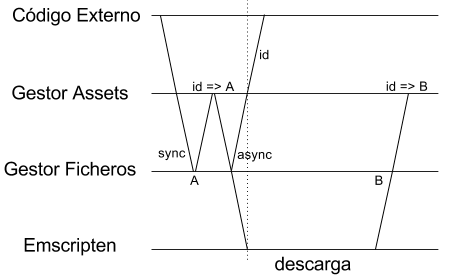
\includegraphics[width=0.60\linewidth]{async_file_manager}
    \caption{Esquema de la carga de ficheros.}
    \label{fig:async_file_manager}
\end{figure}


\cleardoublepage
\chapter{Diseño}
\section{Diseño de software}

\cleardoublepage
\chapter{Desarrollo}


\section{Mallas dinámicas}
\label{walls_holes}
Uno de los principales requerimientos para un planificador es la visualización de paredes y configuración de estas para adaptarlas a las medidas de una estancia. Además, deben poderse ubicar ventanas y puertas en las paredes, lo cual afecta a la geometría de la pared dado que se debe poder ver a través de estos elementos. Para ello no es factible utilizar mallas pregeneradas, se necesita generar las paredes de forma dinámica.

En este apartado se describe el proceso de desarrollo de las paredes en 2 iteraciones, una primera en la que se crea una estructura básica para las paredes, y otra en la que se tienen en cuenta las ventanas y puertas.

%%%%%%%%%%%%%%%%%%%%%%%%%%%%%%%%%%%%%%%%%%%%%%%%%%%%%%%%%%%%%%%%%%%%%%%%%%%%%
%%%%%%%%%%%%%%%%%%%%%%%%%%%%%%%%%%%%%%%%%%%%%%%%%%%%%%%%%%%%%%%%%%%%%%%%%%%%%
%%%%%%%%%%%%%%%%%%%%%%%%%%%%%%%%%%%%%%%%%%%%%%%%%%%%%%%%%%%%%%%%%%%%%%%%%%%%%
\subsection{Generación de la estructura básica de la pared}
\label{subsec:gen1}
El primer paso ha sido crear una definición de los datos que se recibirán para describir cómo ha de ser la pared. Se trata de una lista de puntos en dos dimensiones y un valor booleano que indica si esta lista debe cerrarse conectando el último punto con el primero. Esto último es importante porque, como se puede ver en la figura \ref{fig:vertical_view_walls}, la geometría de una esquina ``suelta" es diferente a la de una esquina que conecta dos paredes entre sí.

\begin{figure}[h]
    \centering
    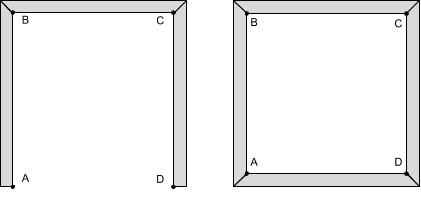
\includegraphics[width=0.65\linewidth]{Vista_Vertical_Paredes}
    \caption{Paredes en vista vertical.}
    \label{fig:vertical_view_walls}
\end{figure}

Estos datos nos permiten no sólo crear habitaciones sino también paredes únicas o incluso otros tipos de estructuras, normalmente interiores, similares a una pared. La intención es que en el futuro el programa pueda utilizarse en otras herramientas para hacer diseños más complicados como el plano de una planta completa de un edificio.

Teniendo en cuenta la estructura de una malla, explicada en el apartado \ref{mesh_light_cam}, en la figura \ref{fig:io_generatewalls} se puede ver la conversión de los datos que se espera conseguir.

\begin{figure}[H]
    \centering
    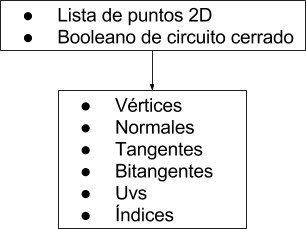
\includegraphics[width=0.5\linewidth]{IO_paredes}
    \caption{Input y output del generador de paredes.}
    \label{fig:io_generatewalls}
\end{figure}

El output está formado por listas de valores planos. Por ejemplo, la lista de vértices está formada por los valores de posición ``x,y,z" de cada uno sucesivamente.

Por cada pared hay tres primeros puntos 2D relevantes: las esquinas izquierda de las paredes anterior, actual, y siguiente. A partir de estos tres puntos puede deducirse la información de la figura \ref{fig:wall_vectors}, donde los vectores ``N1" y ``N2" son las normales de cada pared, siempre hacia el exterior de la estancia.

\begin{figure}[H]
    \centering
    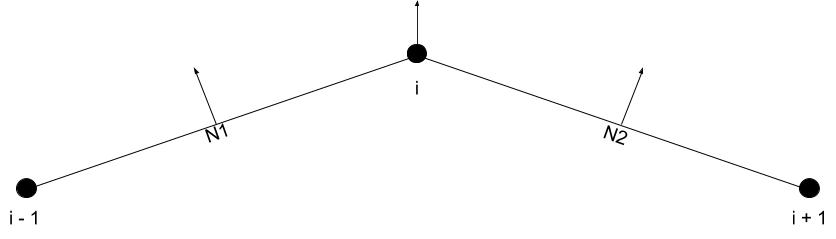
\includegraphics[width=\linewidth]{data_from_3_points}
    \caption{Vectores extraídos a partir de 3 puntos consecutivos.}
    \label{fig:wall_vectors}
\end{figure}

``N1" y ``N2" pueden obtenerse normalizando los vectores de un punto a otro, y girándolos. La dirección del vector central es la suma normalizada de estos dos o, en el caso de las paredes en los extremos cuando el circuito no está cerrado, la normal de la propia pared:

\begin{lstlisting}
VARIABLES EXTERNAS:
    puntos: lista de puntos 2D
    i: punto desde el que queremos obtener las normales de pared
    cerrado: booleano que indica si se quiere cerrar el conjunto de paredes

VARIABLE direccion TIPO VECTOR
VARIABLES v_pc, v_cn, normal_actual, normal_anterior TIPO VECTOR
VARIABLES actual, anterior, siguiente TIPO NUMERO

actual = i
anterior = i - 1

SI i EQUIVALE A tamaño(puntos) ENTONCES:
    siguiente = 0
SINO
    siguiente = i + 1
FINSI

v_pc = puntos[actual] - puntos[anterior];
v_cn = puntos[siguiente] - puntos[actual];

SI cerrado Y (actual EQUIVALE A tamaño(puntos) - 1 O actual EQUIVALE A 0) ENTONCES:
    normal_actual = GIRAR 90 GRADOS ANTI-HORARIO v_cn Y NORMALIZAR
    direccion = puntos[actual] + normal_actual
SINO
    normal_actual = GIRAR 90 GRADOS ANTI-HORARIO v_cn
    normal_anterior = GIRAR 90 GRADOS ANTI-HORARIO v_pc
    direccion = normal_actual + normal_anterior
    NORMALIZAR direccion
FINSI
\end{lstlisting}

Por último se debe tener en cuenta el grosor que se espera que tenga la pared, dado que si se avanza siempre la misma distancia en el vector director el grosor de estas dependería del ángulo que formen con sus paredes adyacentes. Esto se resuelve con trigonometría:

\begin{lstlisting}
SI cerrado ENTONCES:
    direccion = profundidad_pared / absoluto(producto_punto(normal_actual, direccion));
SINO
    direccion = profundidad_pared * normal_actual
FINSI

punto_esquina = puntos[actual] + direccion
\end{lstlisting}

El producto punto de dos vectores normales es el coseno del ángulo que forman entre sí. En este momento ``direccion" incluye la dirección y distancia entre el punto actual y el punto de la esquina exterior, permitiendo generar dicho punto a partir del actual. En el caso de que la pared que estamos generando no haga esquina con otra, simplemente se utiliza la normal de la pared actual.

Una limitación de este sistema es que los puntos deben introducirse en sentido anti-horario respecto al interior de la habitación. De lo contrario la normal de cada pared queda invertida y estas se extienden hacia el lado opuesto al que deberían, provocando algunos artefactos no deseados.

%%%%%%%%%%%%%%%%%%%%%%%%%%%%%%%%%%%%%%%%%%%%%%%%%%%%%%%%%%%%%%%%%%%%%%%%%%%%%
%%%%%%%%%%%%%%%%%%%%%%%%%%%%%%%%%%%%%%%%%%%%%%%%%%%%%%%%%%%%%%%%%%%%%%%%%%%%%
%%%%%%%%%%%%%%%%%%%%%%%%%%%%%%%%%%%%%%%%%%%%%%%%%%%%%%%%%%%%%%%%%%%%%%%%%%%%%
\subsection{Índices para la estructura básica}
Para referir a cada uno de los vértices se ha definido la nomenclatura ``A, B, A2, B2" como puede verse en la figura \ref{fig:nomenclatura_vertices}, además de los correspondientes ``AH, BH, A2H, B2H" en la parte alta de la pared. Posteriormente, los índices de la pared se extraen de los que habría normalmente en un cubo, aprovechando que sus vértices se conectan del mismo modo.

\begin{figure}[H]
    \centering
    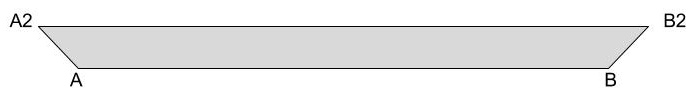
\includegraphics[width=0.75\linewidth]{Nomenclaturas_vertices}
    \caption{Nomenclatura básica de los vértices.}
    \label{fig:nomenclatura_vertices}
\end{figure}

La pared tiene 23 vértices y no 8 como cabría esperar. Esto se debe a que al renderizar, los shaders interpolan la normal de cada vértice con la de sus vecinos; si el mismo vértice se encuentra en dos caras distintas, la normal del vértice no coincide con la de la superficie en la cara que se está pintando. El resultado de esto sería que el color varía en los bordes de cada cara. Esta propiedad es muy útil para objetos que no tienen ángulos tan marcados, pero en este caso se busca que las caras sean muy marcadas y totalmente planas.

Para solucionarlo se repite cada vértice tantas veces como el número de caras en el que se encuentre, de modo que aunque todos se encuentren en la misma posición, cada cara está utilizando un vértice distinto.

\begin{figure}[H]
    \centering
    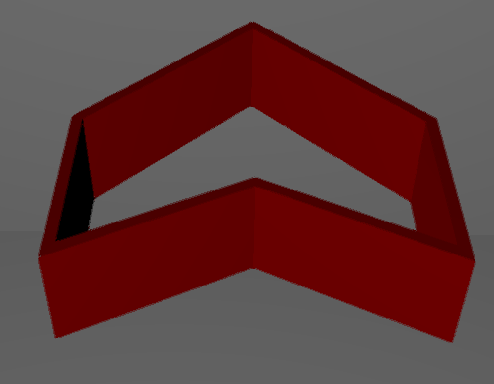
\includegraphics[width=0.75\linewidth]{paredes_first}
    \caption{Ejemplo de generación de paredes.}
    \label{fig:paredes_first}
\end{figure}

%%%%%%%%%%%%%%%%%%%%%%%%%%%%%%%%%%%%%%%%%%%%%%%%%%%%%%%%%%%%%%%%%%%%%%%%%%%%%
%%%%%%%%%%%%%%%%%%%%%%%%%%%%%%%%%%%%%%%%%%%%%%%%%%%%%%%%%%%%%%%%%%%%%%%%%%%%%
%%%%%%%%%%%%%%%%%%%%%%%%%%%%%%%%%%%%%%%%%%%%%%%%%%%%%%%%%%%%%%%%%%%%%%%%%%%%%
\subsection{Modificando la estructura para permitir la inclusión de ventanas}
\label{subsec:gen2}
El siguiente paso es implementar la posibilidad de añadir puertas y ventanas a la estancia. Insertar el modelo correspondiente en cada caso no será un problema, pero para que el efecto sea convincente es necesario poder ver a través de estos. Eso implica que se debe que modificar la geometría de las paredes para que incluya huecos donde tengan que ir dichas ventanas y puertas.

Del mismo modo que con las paredes inicialmente, se define un input: por cada hueco existe un punto 3D (que como se verá a continuación, no necesariamente debe colisionar con una pared), una altura y un ancho. El input/output del algoritmo completo para generar paredes quedaría como se puede ver en la figura \ref{fig:io_generatewindows}.

\begin{figure}[H]
    \centering
    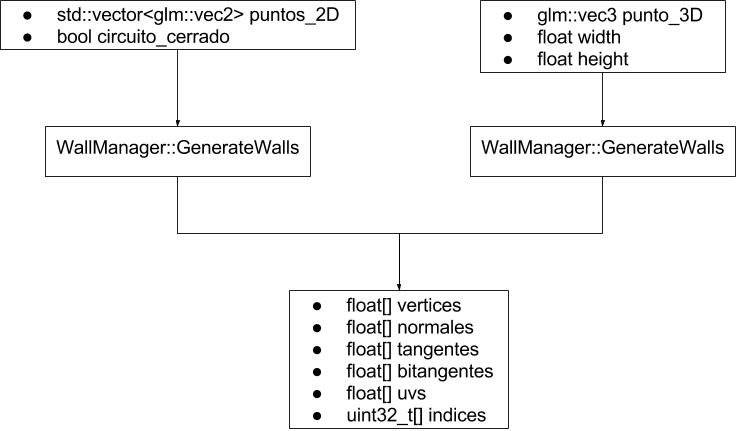
\includegraphics[width=0.75\linewidth]{I_O_ventanas}
    \caption{Nuevo input y output de GenerateWalls, incluyendo ventanas.}
    \label{fig:io_generatewindows}
\end{figure}

Para empezar se deben adaptar las paredes que ya generadas. Es conveniente que la generación de ventanas se limite a trabajar sobre un solo plano, de modo que se eliminarán los planos anterior y posterior de la pared para añadirlos después con la nueva geometría. Aunque intuitivamente pueda parecer que esto supone simplificar la geometría respecto a lo que se ha hecho hasta ahora, en realidad se complica sensiblemente. Los planos anterior y posterior de la pared van a ser siempre idénticos, pero el plano posterior es algo más alargado debido a la geometría de las esquinas que se puede apreciar en la figura \ref{fig:nomenclatura_vertices}.

\begin{figure}[H]
    \centering
    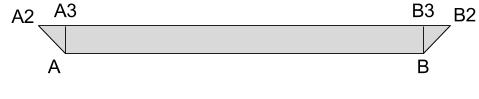
\includegraphics[width=0.75\linewidth]{Nomenclaturas_vertices_2}
    \caption{Nomenclatura final de los vértices.}
    \label{fig:nomenclatura_vertices_2}
\end{figure}

Con la nueva geometría presentada en la figura \ref{fig:nomenclatura_vertices_2} las paredes se convierten en dos prismas triangulares unidos por dos planos superior e inferior de la pared. Con esto se consigue que los planos anterior y posterior que ahora le faltan a la pared sean totalmente idénticos aunque con las normales invertidas. Esto, sin embargo, complica las conexiones entre los vértices, que se han tenido que generar manualmente. Con los nuevos vértices añadidos en total hay 35 vértices.

\begin{figure}[H]
    \centering
    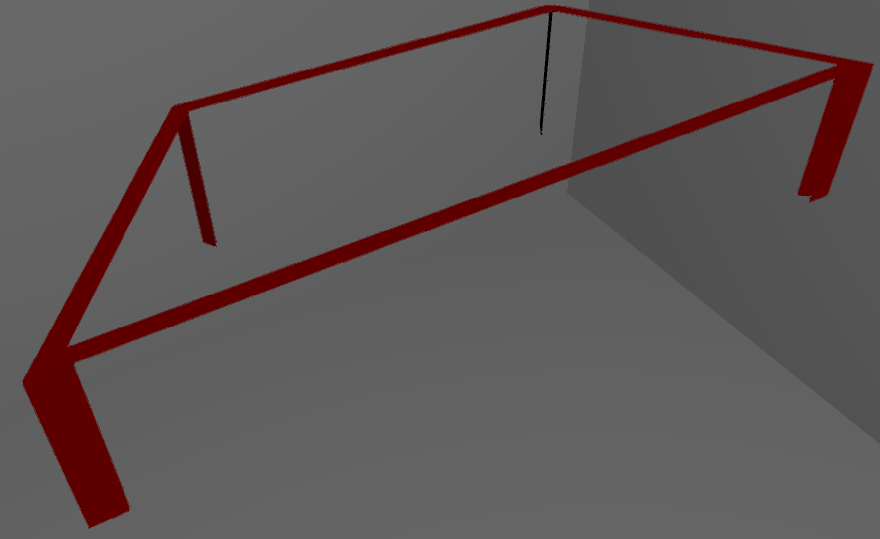
\includegraphics[width=0.75\linewidth]{paredes_frame}
    \caption{Aspecto de las paredes sin los planos anterior y posterior.}
    \label{fig:nueva_estructura}
\end{figure}

En la figura \ref{fig:nueva_estructura} puede verse el resultado. Nótese que los planos inferiores no se ven porque sus normales apuntan hacia abajo y el motor gráfico los oculta como optimización. Al crear los índices se ha tenido en cuenta el orden de estos, pues afecta al cálculo de las normales de los vértices.

%%%%%%%%%%%%%%%%%%%%%%%%%%%%%%%%%%%%%%%%%%%%%%%%%%%%%%%%%%%%%%%%%%%%%%%%%%%%%
%%%%%%%%%%%%%%%%%%%%%%%%%%%%%%%%%%%%%%%%%%%%%%%%%%%%%%%%%%%%%%%%%%%%%%%%%%%%%
%%%%%%%%%%%%%%%%%%%%%%%%%%%%%%%%%%%%%%%%%%%%%%%%%%%%%%%%%%%%%%%%%%%%%%%%%%%%%
%\clearpage
\subsection{Generación de ventanas I: proyección sobre pared}
\label{sec:wallgenwindowsi}
Como ya se ha mencionado en el apartado \ref{subsec:gen2}, las ventanas están definidas por un punto, una altura y un ancho. No se incluye ninguna información respecto a que pared es la que va a contener dicha ventana; por lo que se cogerá la pared más cercana al punto dado.

Para ello se proyecta el punto sobre la línea $AB$ de cada una de las paredes, calculando la distacia hasta cada una de las proyecciones para ver cuál es la más cercana (véase el apéndice \ref{sec:pointrayproj} sobre la proyección punto-línea):

\begin{lstlisting}
findWall(punto):
    VARIABLE pared_proxima
    VARIABLE distancia_menor
    VARIABLE distancia
    
    pared_proxima = -1
    distancia_menor = -1.0
    
    POR CADA ELEMENTO EN paredes, i:
        VARIABLE proyeccion
        proyeccion = proyeccion_punto_linea(pared[i].A1, pared[i].B1, punto)
        
        SI proyeccion encontrada ENTONCES:
            distancia = LOGITUD DE VECTOR (proyeccion - punto)
            SI distancia_menor ES MENOR QUE 0.0 O distancia < distancia_menor ENTONCES:
                distancia_menor = distancia
                pared_proxima = i
            FINSI
        FINSI
    FINPOR
    DEVOLVER pared_proxima
FIN DE FUNCION
\end{lstlisting}

Todas las ventanas o puertas han de ser necesariamente rectangulares. Esta es una precondición que se ha impuesto desde desarrollo para simplificar el cálculo de los agujeros, dado que es más sencillo incorporar geometrías más complejas incluyendo paredes falsas dentro del modelo de la ventana o puerta. Por ejemplo, si en algún momento se deseara incorporar una ventana redonda, sería más sencillo incluir 4 esquinas de pared a la ventana permitiendo que el hueco sea rectangular igualmente.

Como preparación para el próximo apartado (\ref{sec:wallgenwindowsii}) se calcula sobre la pared los 4 puntos que delimitarán la ventana. Para ello se proyecta el punto de la pared sobre el plano que forma esta, y se calcula el resto de puntos desplazándonos por dicho plano (véase el apéndice \ref{sec:pointplaneproj} sobre la proyección punto-rectángulo):

\begin{lstlisting}
projectVertices(pared, referencia a hueco):
    VARIABLE direccion_A1B1
    VARIABLE direccion_A1A1H
    VARIABLE origen
    
    direccion_A1B1 = NORMALIZAR (pared.B1 - pared.A1)
    direccion_A1A1H = NORMALIZAR (pared.A1H - pared.A1)
    
    origen = proyeccion_punto_rectangulo(pared.A1, pared.B1, pared.A1H, hueco.origen)
    
    hueco.A1 = origen
    hueco.B1 = origen + direccion_A1B1 * hueco.ancho
    hueco.A1H = origen + direccion_A1A1H * hueco.alto
    hueco.B1H = hueco.A1H + direccion_A1B1 * hueco.ancho
FIN DE FUNCION
\end{lstlisting}

%%%%%%%%%%%%%%%%%%%%%%%%%%%%%%%%%%%%%%%%%%%%%%%%%%%%%%%%%%%%%%%%%%%%%%%%%%%%%
%%%%%%%%%%%%%%%%%%%%%%%%%%%%%%%%%%%%%%%%%%%%%%%%%%%%%%%%%%%%%%%%%%%%%%%%%%%%%
%%%%%%%%%%%%%%%%%%%%%%%%%%%%%%%%%%%%%%%%%%%%%%%%%%%%%%%%%%%%%%%%%%%%%%%%%%%%%
\subsection{Generación de ventanas II: modificación de la geometría de la pared}
\label{sec:wallgenwindowsii}

Al final del apartado \ref{sec:wallgenwindowsii}, ya se conoce el punto en que están los extremos de la ventana sobre la pared. En este apartado se explica cómo dividir la pared en diferentes planos y descartar aquellos que correspondan a un agujero.

Una vez más las proyecciones cobran mucho protagonismo (véase el apéndice \ref{sec:pointrayproj} sobre la proyección punto-línea). Lo primero que se busca es dividir el plano de la pared por los vértices del hueco, obteniendo una colección de planos como se puede ver en la figura \ref{fig:wall_separacion}.

\begin{figure}[H]
    \centering
    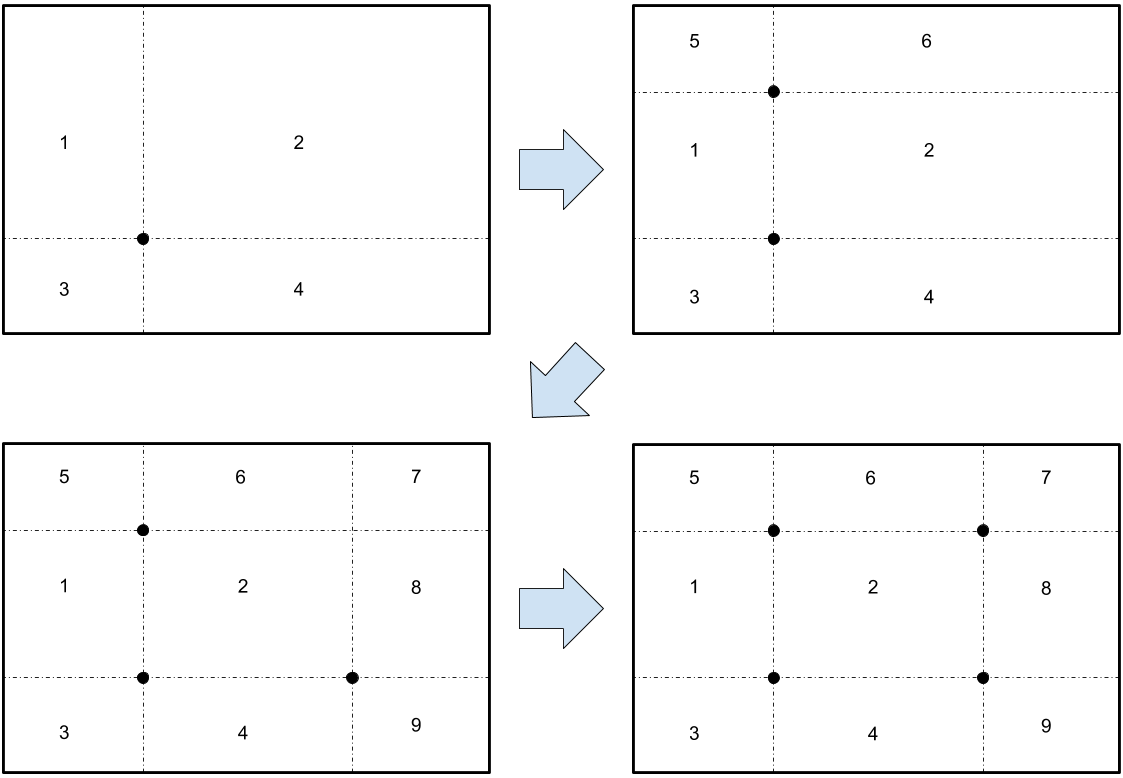
\includegraphics[width=0.85\linewidth]{Separaciones_paredes}
    \caption{Separación de la pared en planos}
    \label{fig:wall_separacion}
\end{figure}

El algoritmo para conseguir esto tiene como entrada y salida una lista de planos, que empieza siendo uno solo que cubre toda la pared. Mientras iteramos los puntos, proyectamos estos sobre cada lado para obtener los puntos por los que hay que cortar los planos, y posteriormente se añaden a la lista de planos desechando el original. En caso de que una de las proyecciones no contribuya a crear un nuevo plano (como por ejemplo, los puntos inferiores de la puerta en la figura \ref{fig:mult_and_red_windows}) la ignoramos.

Posteriormente se comprueba cuales de estos planos forman parte de una ventana y se eliminan de la lista, dejando un hueco en dicha posición. Este algoritmo permite además añadir múltiples ventanas, aumentando la posible complejidad de la pared.

Por último se reprocesan los planos generados comprobando si sus lados coinciden en alguna dirección, en cuyo caso se reúnen para reducir la complejidad. En la figura \ref{fig:mult_and_red_windows}, se puede ver un ejemplo de como se separan los planos con múltiples ventanas, y cómo se reúnen los planos adyacentes.

\begin{figure}[H]
    \centering
    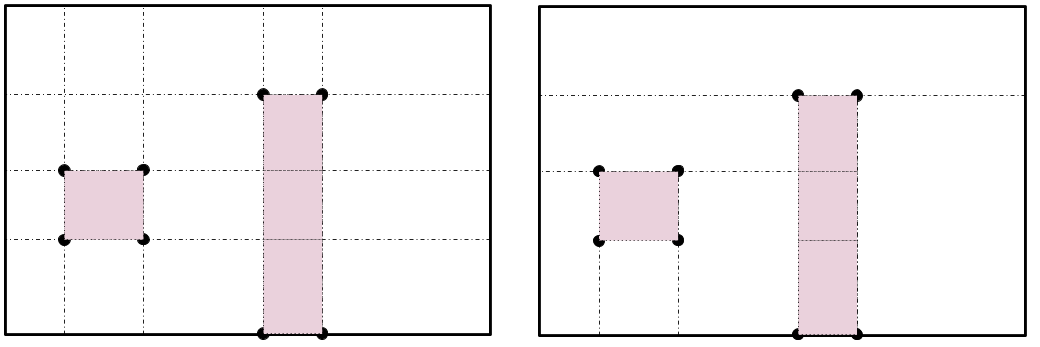
\includegraphics[width=0.85\linewidth]{mult_window_and_reduction}
    \caption{Ejemplo de pared con una ventana y una puerta, y muestra de una posible reducción de los planos.}
    \label{fig:mult_and_red_windows}
\end{figure}

\begin{figure}[H]
    \centering
    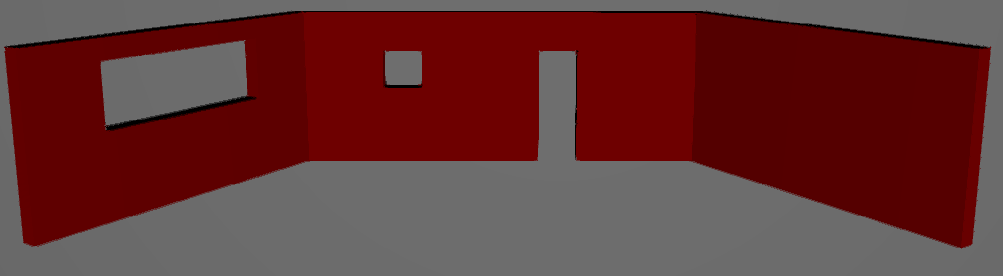
\includegraphics[width=0.85\linewidth]{Agujeros}
    \caption{Ejemplo de generación de paredes con huecos y estancia sin cerrar.}
    \label{fig:wall_with_window_example}
\end{figure}

%%%%%%%%%%%%%%%%%%%%%%%%%%%%%%%%%%%%%%%%%%%%%%%%%%%%%%%%%%%%%%%%%%%%%%%%%%%%%
%%%%%%%%%%%%%%%%%%%%%%%%%%%%%%%%%%%%%%%%%%%%%%%%%%%%%%%%%%%%%%%%%%%%%%%%%%%%%
%%%%%%%%%%%%%%%%%%%%%%%%%%%%%%%%%%%%%%%%%%%%%%%%%%%%%%%%%%%%%%%%%%%%%%%%%%%%%
\subsection{Generación de uvs}
Para que el motor aplique correctamente las texturas sobre las paredes, se requiere que las uvs estén a escala de mundo; es decir, se espera que dada una distancia entre dos vértices de la mima malla, sus uvs tengan la misma distancia. La mayor dificultad en este caso está en que los vértices se encuentran en espacio tridimensional, mientras que las uv son coordenadas bidimensionales de la textura que estamos mapeando. Por lo tanto, de algún modo hay que desconsiderar la orientación de la pared y centrarnos en sus superficies.

Como la geometría está formada por planos perfectos, la solución encontrada ha consistido en partir siempre de la esquina inferior izquierda de cada uno de ellos. Como precondición, la esquina ``A" tiene la uv (0,0).

Por lo tanto por cada plano, se ha definido la uv de la esquina inferior izquierda, y los vectores hacia los cuales ``avanzan" las componentes \texttt{x} e \texttt{y} de las uv (Fig. \ref{fig:datos_uvs}).

\begin{figure}[H]
    \centering
    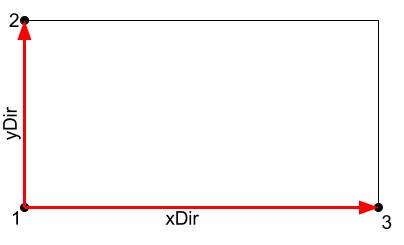
\includegraphics[scale=0.75]{Datos_uvs}
    \caption{Datos necesarios para la generación de las uv ``2" y ``3".}
    \label{fig:datos_uvs}
\end{figure}

La razón de usar proyecciones y no la magnitud de los vectores directamente, es que se desconoce en cual de las dos direcciones se encuentra el vértice que observamos al iterar. Proyectando cada punto tenemos la distancia en cada una de las dos direcciones y se la sumamos a la uv del vértice ``1":

\begin{lstlisting}
genUV(origen, xDir, yDir, punto, uv_origen, longitud_x, longitud_y):
    VARIABLE uv COMO VECTOR 2D
    uv.x = proyeccion_punto_rayo(origen, xDir, punto)
    uv.y = proyeccion_punto_rayo(origen, yDir, punto)
    
    SI longitud_x > 0.0 Y uv.x < 0.0 ENTONCES:
        uv.x = longitud_x - uv.x
    FINSI
    SI longitud_y > 0.0 Y uv.y < 0.0 ENTONCES
        uv.y = longitud_y - uv.y
    FINSI
    
    uv = uv + uv_origen
    DEVOLVER uv
FIN DE FUNCION
\end{lstlisting}

Dado que las uv no pueden ser negativas, se hace un paso en las líneas 6-11 para que, en caso de serlo, se les sume la longitud total del lado en el que se encuentran.

%%%%%%%%%%%%%%%%%%%%%%%%%%%%%%%%%%%%%%%%%%%%%%%%%%%%%%%%%%%%%%%%%%%%%%%%%%%%%
%%%%%%%%%%%%%%%%%%%%%%%%%%%%%%%%%%%%%%%%%%%%%%%%%%%%%%%%%%%%%%%%%%%%%%%%%%%%%
%%%%%%%%%%%%%%%%%%%%%%%%%%%%%%%%%%%%%%%%%%%%%%%%%%%%%%%%%%%%%%%%%%%%%%%%%%%%%
\subsection{Generación de normales, tangentes y bitangentes}
El cálculo de cada normal es el resultado de la suma de la normal de cada polígono en el que se encuentra dicho vértice, y para calcular esta se hace el producto vectorial (normalizado) de los vectores que van del primer vértice hacia el segundo y el tercero:

\begin{lstlisting}
VARIABLES EXTERNAS v1, v2, v3

normal = NORMALIZAR ( PRODUCTO CRUZADO DE (v2 - v1) Y (v3 - v1))
\end{lstlisting}

Las tangentes y bitangentes son un poco más complicadas: todo vector tiene infinitos vectores tangentes, pero en este caso no sirve cualquiera. El vector tangente a la normal tiene que estar siempre alineado con las uv.

Como se explica en el tutorial 13 de opengl-tutorial.org \footfullcite{opengltutorials}, para ello debemos resolver el siguiente sistema de ecuaciones:


\[ deltaPos1 = deltaUV1.x * T + deltaUV1.y * B \]
\[ deltaPos2 = deltaUV2.x * T + deltaUV2.y * B \]

Esto se computar como

\begin{lstlisting}
VARIABLES EXTERNAS uv1, uv2, uv3, v1, v2, v3

VARIABLES vec1, vec2
vec1 = v2 - v1
vec2 = v3 - v1

VARIABLES deltaUV1, deltaUV2 COMO VECTORES 2D
deltaUV1 = uv2 - uv1
deltaUV2 = uv3 - uv1

VARIABLE r
r = 1.0 / (deltaUV1.x * deltaUV2.y - deltaUV1.y * deltaUV2.x)

VARIABLES tangente, bitangente
tangente = (vec1 * deltaUV2 - vec2 * deltaUV1.y) * r
bitangente = (vec2 * deltaUV1.x - vec1 * deltaUV2.x) * r
\end{lstlisting}

\section{Interacción}
En este apartado se darán algunos detalles sobre cómo se ha implementado la interacción del usuario con la aplicación.

\subsection{Gestión de los inputs y uso del Patrón Estado}
El motor gráfico Manta tiene una interfaz para configurar los inputs. Se puede definir la función que debe llamarse cuando se da un evento de input determinado.

Como se ha explicado en el capítulo \ref{app_design}, los inputs se redirigen al estado de la aplicación que esté activo en ese momento a través de \texttt{World}. Durante el desarrollo los estados utilizados han sido: \texttt{StandardView}, \texttt{OverView} y \texttt{LateralView}. Podrían definirse más estados en futuros desarrollos.

Cada estado configura la cámara en su método \texttt{In}. \texttt{OverView} y \texttt{LateralView} configuran la cámara a modo ortogonal y la sitúan en frente del elemento que se quiere mostrar: una vista hacia abajo de toda la habitación en el caso de \texttt{OverView} y una vista frontal de cada una de las paredes en el caso de \texttt{LateralView}. Por su parte, \texttt{StandardView} tiene una cámara libre que puede moverse por el usuario final.

El estado más complejo es \texttt{OverView}, desde el cual puede modificarse la estancia. Las paredes pueden moverse arrastrando una pared en sí o su esquina, en ambos casos afectando también a las paredes que estén conectadas.

Al hacer click, el método \texttt{OnMouseClick} se llama con la posición del click como parámetro. Para saber en que elemento se ha hecho click, los vértices de cada una de las paredes se transforman a coordenadas de pantalla usando las matrices de vista y perspectiva de la cámara. Los vértices superiores de la pared forman un rectángulo en dos dimensiones que puede compararse con la posición del ratón. A su vez, calculando la distancia entre la posición del ratón y la de los vértices en las esquinas puede saberse si se ha clickado en una esquina. Una vez detectado el elemento con el que se está interactuando se guarda su identificador en el estado, y un booleano que indica que el ratón se está manteniendo pulsado.

Mientras el booleano siga activado, el método \texttt{OnMouseMove} del estado mandará la posición del ratón y el elemento seleccionado al framework de la aplicación (véase el apartado \ref{engine_design}), que procesará el modo en que reaccionan los elementos de la escena a la interacción. La respuesta del framework a ese proceso se utilizará para regenerar las paredes.

Para permitir que esto ocurra en tiempo real se utilizarán comandos, como se explica en el apartado \ref{use_of_command}.

\subsection{Uso del Patrón Comando}
\label{use_of_command}
El Patrón Comando, explicado en el apartado \ref{command_pattern}, permite definir distintas acciones y contra-acciones para la aplicación.

Toda la interacción con el gestor de paredes y huecos se ha realizado a través de comandos. Por lo tanto, la aplicación permite hacer y deshacer acciones como mover, añadir o eliminar paredes y huecos.

Un defecto del Patrón Comando es que requiere crear una instancia cada vez que se realiza un comando. Esto puede ser un problema cuando estamos interactuando con el programa de forma constante, como por ejemplo moviendo una pared con el ratón. No es viable crear una instancia de un comando cada vez que el ratón se mueve un píxel en la pantalla, y además no tiene sentido poder deshacer una acción si esta se ha realizado un gran número de veces para mover un poco algún elemento.

Para solucionarlo, se ha añadido el métodoi \texttt{Update} sólo a los comandos que requerían una actualización constante durante un tiempo determinado. La instancia del comando se crea con la información del elemento a modificar, y guardando el estado previo, pero la acción en sí se realiza con el método \texttt{Update} en vez de \texttt{Do}. Al llamar a \texttt{Update} no se guarda la acción en el historial, por lo que podemos realizarla todas las veces que sea necesario; cuando la acción termine (normalmente, cuando el usuario suelte el ratón), se llama al método \texttt{Do} para que la acción quede registrada.

Con este sistema se registra una sola acción para algo que realmente se ha hecho muchas veces en un período de tiempo. Si se deshace la acción se volverá al estado previo a empezar la acción.

Otros casos como añadir y eliminar elementos no han necesitado esta complejidad añadida.

\cleardoublepage
\chapter{Conclusiones}
\section{Estado actual del desarrollo}
Para el desarrollo de la interfaz en la versión actual de la aplicación se ha hecho uso de la librería ImGui\footfullcite{imgui}. Se trata de una API que permite añadir diversos tipos de elementos de interfaz en la aplicación. Aunque es muy fácil de utilizar y versátil, probablemente será insuficiente de cara a la versión en producción de la aplicación: ImGui está altamente enfocado a interfaces de debugging y los requisitos estéticos de los planificadores no podrán cumplirse fácilmente. Será necesario buscar alternativas, por lo que de momento ImGui sólo se utiliza para debugging.

Una posible alternativa, al menos como paso intermedio antes de crear una interfaz más avanzada dentro del canvas 3D, es integrar la interfaz dentro del HTML. El buen funcionamiento de la aplicación en web hace que ya sea posible empezar a desarrollar la interfaz de usuario en HTML, utilizando la comunicación entre C++ y Javascript. Es una buena opción para empezar a trabajar en la interfaz sin interrumpir el desarrollo de la propia aplicación.

Al comenzar el desarrollo existía cierto escepticismo sobre las posibilidades de Emscripten. Llevar código de lenguajes de escritorio a plataformas web hasta hace poco ha sido algo muy poco común, a excepción de algunos plug-ins de navegador con muy poca recepción. Las primeras pruebas con Emscripten resultaron sorprendentes y eso fue un aliciente.

A pesar de ello, durante el desarrollo y la exportación del código con Emscripten han habido muchos problemas. Los más importantes han sido:

\begin{itemize}
    \item La compilación de código de C++ a Javascript es considerablemente lenta, hasta aproximadamente 5 minutos. En los momentos en los que han surgido dificultades específicas de Javascript o Emscripten esto ha ralentizado el desarrollo, puesto que se han necesitado varias iteraciones hasta dar con la combinación correcta de elementos. Aunque las interrupciones solo sean de 5 minutos la pérdida de tiempo productivo puede ser mucho mayor en muchos casos. Debido a esto la mayor parte del desarrollo se ha realizado debugando primero en escritorio, y no se ha empezado a probar en Emscripten hasta tener muy avanzado el código.

    \item Las diferencias entre la naturaleza síncrona de C++ y asíncrona de Javascript han generado dificultades. Las primeras aproximaciones para ejecutar el motor en web incluían el bucle de ejecución dentro del código C++, provocando el bloqueo de la aplicación. Esto ha afectado especialmente a la gestión de ficheros.

    \item La exportación del sistema de ficheros tiene un gran número de consideraciones a tener en cuenta. Aunque Emscripten ofrece herramientas muy efectivas para la carga de ficheros tanto síncrona como asíncrona, implementar dicha carga sin irrumpir demsiado en el comportamiento del motor gráfico ha sido difícil. El apartado \ref{emscripten_filesistem} sobre la implementación del sistema de ficheros en Emscripten es el resultado de varias iteraciones según surgían problemas inesperados. Por suerte, la posibilidad de cargar assets ``dummys" ha facilitado una solución al problema de la asincronía.
    
    \item La implementación del Patrón Comando, explicada en el apartado \ref{use_of_command} también es el resultado de varios intentos. El desconocimiento del patrón hizo que no se tuvieran en cuenta diversos detalles, como la necesidad de realizar acciones sin registrarlas en el historial o agrupar en un solo comando un conjunto de acciones cuando estas ocurren en tiempo real. La flexibilidad que ofrece la herencia de C++ hace que muchas soluciones puedan aplicarse directamente en los comandos, pero ello requiere conocer dichas soluciones por lo que la creación de comandos no está carente de cierta complejidad.
    
    \item La generación de mallas dinámicas ha tenido un gran número de detalles que no se habían tenido en cuenta al comenzar el desarrollo. El motor no estaba preparado para la actualización de mallas dinámicas y fue necesario añadir dicha funcionalidad, tanto en su versión de escritorio como en WebGL. El desarrollo se empezó sin disponer de dicha funcionalidad pero se pudo avanzar generando ficheros dinámicamente y leyéndolos al instante. Ha habido un gran número de pequeños bugs que han ralentizado el proceso. Se ha necesitado tener una gran cantidad de código antes de poder empezar a probarlo. Puede considerarse un acierto haber realizado el desarrollo de forma iterativa, puesto que no tenía sentido empezar a generar huecos dentro de las paredes sin tener funcionando una versión básica de estas.
    
    \item Ha habido pequeñas diferencias entre la API de OpenGL ES 2 y WebGL que han sido difíciles de solucionar. Un ejemplo es que OpenGL ES 2 permite asignar a un mismo buffer dos targets diferentes, lo cual fue un error en el código pero no hacía fallar la aplicación, mientras que en WebGL sí. En este punto se han unido varios factores como la falta de conocimiento sobre la API, la dificultad de debugar Emscripten, la poca cantidad de gente que se ha encontrado con problemas similres en Internet (el uso de Emscripten aún no está muy extendido) y la extensión del código del motor gráfico, que hace difícil encontrar los puntos específicos donde se produce un error.
\end{itemize}

Tras esta experiencia no se puede afirmar categóricamente que Emscripten sea la mejor alternativa para todas las situaciones, hay que recordar que Javascript también puede trasladarse a otras plataformas; pero Emscripten ha demostrado ser perfectamente capaz de trasladar código C++ a Javascript, y ejecutarlo con la misma estabilidad y una eficiencia muy similar.

Aunque la interfaz de usuario deja mucho que desear, el código es capaz de añadir, mover y eliminar paredes así como añadir, mover y eliminar huecos en estas. Todas las acciones pueden deshacerse y rehacerse, lo cual es una característica que nunca había existido en ninguna aplicación de la empresa.

Ha sido muy satisfactorio ver los buenos resultados de realizar un diseño preliminar, incluyendo la decisión de utilizar patrones. El código ha ganado calidad y mantenibilidad gracias a ello.

Por otro lado, el código tiene margen de mejora en cuanto a los gestores y generadores de entidades, explicados en el apartado \ref{managers}. Muchas de las buenas ideas introducidas en este apartado (como el uso de identificadores para que no se manipulen los datos desde fuera) se han incorporado a mitad del desarrollo y con bastante prisa. El resultado es que en su estado actual, mantener este fragmento de código requiere entender muy bien lo que hace. No debería ser difícil sin embargo, una vez conocidos los problemas y sus soluciones, mejorar este fragmento, pues está muy aislado del resto del código.

El hecho de ser un proyecto en empresa ha aportado ventajas y desventajas al desarrollo. Por un lado es difícil coordinar las prioridades de desarrollo con las prioridades del departamento de ventas. Ha habido mucha presión para tener resultados rápidamente a menudo en detrimento de la calidad del código. Existe una cierta deuda técnica en el código que pasará factura en el futuro. Por contra, trabajar en una empresa ha hecho contar con el apoyo de compañeros con muchos conocimientos sobre la materia. El motor gráfico es propio de la empresa y no se puede buscar información sobre este en Internet pero no solo se ha contado con ayuda para el desarrollo sino que incluso se ha podido adaptar el propio motor a las necesidades que han surgido. El hecho de tratarse de un proyecto real que será utilizado por una gran empresa eventualmente es un gran componente motivador, además del aliciente económico y la presión, aunque a priori no es una experiencia agradable, ayuda a no dormirse. Tener un horario estable de ocho horas diarias ha hecho que los avances fueran constantes y estables.

Habría sido deseable que más personas participaran directamente en el desarrollo de la aplicación. En un principio el equipo iba a estar formado por 3 personas además del equipo que programa el motor. Al final la presión de otros proyectos de la empresa ha hecho que solo hubiera un programador de en la mayor parte del desarrollo y eso ha afectado negativamente las previsiones iniciales.

Estos inconvenientes sin embargo han ido acompañados de comprensión por parte de la empresa, y una readaptación de las expectativas. En términos globales puede decirse que el balance de trabajar en un proyecto de empresa es más que positivo.

\section{Futuras iteraciones}
La adición de elementos interiores e interacción con estos no está terminada, aunque ya se sabe cómo se van a organizar estos elementos (véase el apartado \ref{managers}). Tampoco está hecha la interfaz de usuario y los inputs deben pulirse. Estas serán las prioridades en el futuro inmediato.

A más largo plazo, se deben implementar las diferentes aplicaciones que van a hacer uso del planificador. Se requerirá hacer aplicaciones con múltiples habitaciones y elementos estructurales como posiblemente zonas exteriores (balcones, terrazas o jardines). El planteamiento de diseñar el planificador para ser genérico hará que esto se pueda hacer con relativamente poco esfuerzo. Teniendo en cuenta que la empresa trabaja con diferentes aplicaciones en ambientes muy diferentes, hacer una aplicación genérica ha sido un acierto de cara al futuro.

Es probable que, una vez conocidos los problemas que se han encontrado a lo largo del desarrollo, se de otra iteración a algunos fragmentos del código, para mejorar la eficiencia y la estructura del propio código. Estos fragmentos se han desarrollado con prisa y asumiendo una cierta deuda técnica. Sin embargo, el diseño modular de la aplicación hace que sea posible realizar estas iteraciones trabajando con fragmentos aislados de código.

En su conjunto, la mantenibilidad del código es bastante buena y deberían poder incorporarse nuevos desarrolladores sin excesivo esfuerzo. Algunos fragmentos de código, en cambio, requieren un conocimiento más profundo del problema y de los elementos que intervienen en la solución. Un desarrollador descuidado podría llegar a tener problemas con dichos fragmentos por lo que existe margen de mejora en este aspecto.

\cleardoublepage
\appendix
\chapter{Utilidades matemáticas}
Normalmente un motor gráfico incluye una serie de herramientas para facilitar el desarrollo, pero debido algunas carencias del motor Manta en este aspecto, se han programado como parte de la aplicación. Este apéndice se presenta como referencia para los fragmentos de código que hacen uso de estas herramientas a lo largo de este documento, y como muestra del funcionamiento de estas.

%%%%%%%%%%%%%%%%%%%%%%%%%%%%%%%%%%%%%%%%%%%%%%%%%%%%%%%%%%%%%%%
%%%%%%%%%%%%%%%%%%%%%%%%%%%%%%%%%%%%%%%%%%%%%%%%%%%%%%%%%%%%%%%
%%%%%%%%%%%%%%%%%%%%%%%%%%%%%%%%%%%%%%%%%%%%%%%%%%%%%%%%%%%%%%%
\section{Comparación de tipos imprecisos}
En la mayoría de dispositivos los números de coma flotante tienen un cierto nivel de imprecisión. Esto no suele ser un problema porque suelen tener mucha más precisión de la necesaria, y en su defecto hay otras formas de conseguir aún más precisión. El problema es no se pueden comparar dichos números porque rara vez van a ser \textit{exactamente} idénticos. Para ello se han creado las funciones \texttt{compare\_float(n1, n2, precision)} y \texttt{compare\_vec(v1, v2, precision)}.

Estas funciones comparan que el valor absoluto de la diferencia entre los dos números sea inferor a la precisión requerida que por defecto es $0.01$ pero puede configurarse con un parámetro. Como los vectores en glm utilizan números de coma flotante, se hace lo mismo para poder compararlos, pero esta vez comparando sus 3 componentes.

%%%%%%%%%%%%%%%%%%%%%%%%%%%%%%%%%%%%%%%%%%%%%%%%%%%%%%%%%%%%%%%
%%%%%%%%%%%%%%%%%%%%%%%%%%%%%%%%%%%%%%%%%%%%%%%%%%%%%%%%%%%%%%%
%%%%%%%%%%%%%%%%%%%%%%%%%%%%%%%%%%%%%%%%%%%%%%%%%%%%%%%%%%%%%%%
\section{Proyección punto-rayo y punto-línea}
\label{sec:pointrayproj}
Entendiendo un rayo como un elemento formado por un punto y una dirección y una línea como un segmento de un rayo delimitado por dos puntos, se han creado las funciones: 

\begin{lstlisting}
point_ray_projection(origen_rayo, direccion_rayo, punto)
point_line_projection(punto_linea_A, punto_linea_B, referencia resultado) => booleano
\end{lstlisting}

Su funcionamiento es muy similar, de hecho la segunda hace uso de la primera para obtener el resultado, pero tienen dos diferencias importantes: \texttt{point\_ray\_projection} devuelve la distancia entre el origen del rayo y la proyección de nuestro punto, en la dirección especificada, mientras que la función \texttt{point\_line\_projection} devuelve un booleano que indica si la proyección está dentro de nuestra línea, y asigna a la referencia ``result" el punto exacto de la proyección.

Hay diferentes situaciones en las que puede ser más útil una u otra: a veces se querrá saber el punto exacto de la proyección, otras veces la distancia de esta proyección respecto al punto de origen (sin necesidad de calcular el punto), y otras comprobar si esta proyección se encuentra delimitada entre dos puntos.

El cálculo de la proyección rayo-punto se basa en las propiedades del producto punto. A continuación se explica el razonamiento por el cual el producto punto puede usarse para calcular una proyección entre dos vectores.

El producto punto, o producto escalar de dos vectores, cumple la siguiente fórmula:
\[ dot(A,B) = |A||B|*cos(\Theta) \]

Donde $\theta$ es el ángulo que forman los dos vectores. Si asumimos que A es un vector normal (se garantizará normalizandolo desde la propia función), esto se reduce a:
\[ dot(|A|,B) = |B|*cos(\Theta) \]

Si miramos esta ecuación desde el punto de vista trigonométrico, $B$ puede entenderse como la hipotenusa del triángulo que forman $A$, $B$, y el vector de $B$ a la proyección de $B$ en $A$. El coseno, por definición, nos indica el ratio entre el lado contiguo de una esquina y la hipotenusa de un triángulo, por lo que al multiplicarlo por la magnitud de B obtenemos la longitud del lado contiguo, es decir, la distancia entre $A$ y la proyección de $B$.

\[ distancia = dot(direccion, punto - origen) \]

Una vez calculada esta distancia, se puede sacar el punto de proyección con la fórmula:
\[ P = origen + |direccion| * distancia \]

%%%%%%%%%%%%%%%%%%%%%%%%%%%%%%%%%%%%%%%%%%%%%%%%%%%%%%%%%%%%%%%
%%%%%%%%%%%%%%%%%%%%%%%%%%%%%%%%%%%%%%%%%%%%%%%%%%%%%%%%%%%%%%%
%%%%%%%%%%%%%%%%%%%%%%%%%%%%%%%%%%%%%%%%%%%%%%%%%%%%%%%%%%%%%%%
\section{Proyección punto-plano y punto-rectángulo}
\label{sec:pointplaneproj}
De un modo similar al visto en el apartado \ref{sec:pointrayproj}, se calcula la proyección a partir del producto punto.

Para ello debe disponerse de la normal de dicho plano. En el caso de la proyección punto-plano se requiere como parámetro para definir el plano, pero en el caso de la proyección punto-rectángulo la calculará a partir de 3 puntos del plano. Este detalle es importante porque el orden de dichos puntos afectará a la dirección de la normal.

Dados 3 puntos $A$, $B$ y $C$, la normal del plano que forman es el producto vectorial de los vectores que van de un punto hacia los otros dos, normalizados.

\[ normal = |(B - A) \times (C - A)| \]

Proyectando el punto sobre el rayo que forman la normal del plano y un punto cualquiera de este, podemos saber a qué distancia se encuentra el punto de dicho plano. Como disponemos de la normal, podemos invertirla y multiplicarla por la distancia obtenida para extraer la proyección sobre el plano.

\[ distancia = dot(normal, punto - A) \]

\[ P = punto - normal * distancia \]

A diferencia de lo que ocurría en el apartado \ref{sec:pointrayproj}, este método no comprueba que la proyección se encuentre dentro del rectángulo. En el apartado \ref{in_rec} se explica como realizar esta comprobación.


%%%%%%%%%%%%%%%%%%%%%%%%%%%%%%%%%%%%%%%%%%%%%%%%%%%%%%%%%%%%%%%
%%%%%%%%%%%%%%%%%%%%%%%%%%%%%%%%%%%%%%%%%%%%%%%%%%%%%%%%%%%%%%%
%%%%%%%%%%%%%%%%%%%%%%%%%%%%%%%%%%%%%%%%%%%%%%%%%%%%%%%%%%%%%%%
\clearpage
\section{Comprobar si cuatro puntos forman parte del mismo plano}
\label{sec:check4pointplane}
En un espacio de $D$ dimensiones, $D+1$ puntos forman parte del mismo espacio de $D-1$ dimensiones si el determinante de la matriz formada por las posiciones de los puntos organizadas verticalmente es 0 \footfullcite{points_sameplane}. En 3D:

\[
\begin{vmatrix}
& x_1 & x_2 & x_3 & x_4 &\\ 
& y_1 & y_2 & y_3 & y_4 &\\ 
& z_1 & z_2 & z_3 & z_4 &\\ 
& 1   & 1   & 1   & 1   &
\end{vmatrix} = 0
\]

Glm ya dispone de una implementación para calcular el determinante de una matriz por lo que no es necesario profundizar más.

%%%%%%%%%%%%%%%%%%%%%%%%%%%%%%%%%%%%%%%%%%%%%%%%%%%%%%%%%%%%%%%
%%%%%%%%%%%%%%%%%%%%%%%%%%%%%%%%%%%%%%%%%%%%%%%%%%%%%%%%%%%%%%%
%%%%%%%%%%%%%%%%%%%%%%%%%%%%%%%%%%%%%%%%%%%%%%%%%%%%%%%%%%%%%%%
\section{Comprobar si la proyección de un punto sobre un plano está dentro de un rectángulo}
\label{in_rec}
Aunque es similar, este se diferencia del apartado \ref{sec:check4pointplane} en que no se requiere que el punto que queremos comparar esté en el mismo plano que el resto. En algunos casos se desea comprobar si la proyección está dentro de un rectángulo sin importar cuál sea esa proyección.

Para ello utilizamos la proyección punto-línea explicada en el apartado \ref{sec:pointrayproj}. La proyección del punto está dentro del rectángulo si se puede proyectar con éxito sobre sus cuatro lados. Poder proyectarlo sobre un lado implica que se podrá proyectar también sobre el lado opuesto, así que en el fondo solo se necesitan dos comprobaciones.

\begin{lstlisting}
in_rec(A, B, C, punto) => booleano:
    VARIABLES p1, p2 COMO VECTOR
    DEVOLVER
        point_line_projection(A, B, punto, p1) 
        Y 
        point_line_projection(A, B, punto, p2)
FIN DE FUNCION
\end{lstlisting}


%\bibliographystyle{unsrt}
%\bibliography{Bibliography}
\printbibliography

\end{document}